\documentclass[3p]{elsarticle} %review=doublespace preprint=single 5p=2 column
%%% Begin My package additions %%%%%%%%%%%%%%%%%%%
\usepackage[hyphens]{url}

  \journal{Journal of Archaeological Science} % Sets Journal name


\usepackage{lineno} % add
  \linenumbers % turns line numbering on

\usepackage{graphicx}
%%%%%%%%%%%%%%%% end my additions to header

\usepackage[T1]{fontenc}
\usepackage{lmodern}
\usepackage{amssymb,amsmath}
\usepackage{ifxetex,ifluatex}
\usepackage{fixltx2e} % provides \textsubscript
% use upquote if available, for straight quotes in verbatim environments
\IfFileExists{upquote.sty}{\usepackage{upquote}}{}
\ifnum 0\ifxetex 1\fi\ifluatex 1\fi=0 % if pdftex
  \usepackage[utf8]{inputenc}
\else % if luatex or xelatex
  \usepackage{fontspec}
  \ifxetex
    \usepackage{xltxtra,xunicode}
  \fi
  \defaultfontfeatures{Mapping=tex-text,Scale=MatchLowercase}
  \newcommand{\euro}{€}
\fi
% use microtype if available
\IfFileExists{microtype.sty}{\usepackage{microtype}}{}
\bibliographystyle{elsarticle-harv}
\usepackage{graphicx}
\ifxetex
  \usepackage[setpagesize=false, % page size defined by xetex
              unicode=false, % unicode breaks when used with xetex
              xetex]{hyperref}
\else
  \usepackage[unicode=true]{hyperref}
\fi
\hypersetup{breaklinks=true,
            bookmarks=true,
            pdfauthor={},
            pdftitle={Stable isotope approach to farming and husbandry practices at the Phoenician site of Castro Marim between 7th -- 5th century BCE},
            colorlinks=false,
            urlcolor=blue,
            linkcolor=magenta,
            pdfborder={0 0 0}}
\urlstyle{same}  % don't use monospace font for urls

\setcounter{secnumdepth}{5}
% Pandoc toggle for numbering sections (defaults to be off)


% tightlist command for lists without linebreak
\providecommand{\tightlist}{%
  \setlength{\itemsep}{0pt}\setlength{\parskip}{0pt}}

% From pandoc table feature
\usepackage{longtable,booktabs,array}
\usepackage{calc} % for calculating minipage widths
% Correct order of tables after \paragraph or \subparagraph
\usepackage{etoolbox}
\makeatletter
\patchcmd\longtable{\par}{\if@noskipsec\mbox{}\fi\par}{}{}
\makeatother
% Allow footnotes in longtable head/foot
\IfFileExists{footnotehyper.sty}{\usepackage{footnotehyper}}{\usepackage{footnote}}
\makesavenoteenv{longtable}

% Pandoc citation processing
\newlength{\cslhangindent}
\setlength{\cslhangindent}{1.5em}
\newlength{\csllabelwidth}
\setlength{\csllabelwidth}{3em}
\newlength{\cslentryspacingunit} % times entry-spacing
\setlength{\cslentryspacingunit}{\parskip}
% for Pandoc 2.8 to 2.10.1
\newenvironment{cslreferences}%
  {}%
  {\par}
% For Pandoc 2.11+
\newenvironment{CSLReferences}[2] % #1 hanging-ident, #2 entry spacing
 {% don't indent paragraphs
  \setlength{\parindent}{0pt}
  % turn on hanging indent if param 1 is 1
  \ifodd #1
  \let\oldpar\par
  \def\par{\hangindent=\cslhangindent\oldpar}
  \fi
  % set entry spacing
  \setlength{\parskip}{#2\cslentryspacingunit}
 }%
 {}
\usepackage{calc}
\newcommand{\CSLBlock}[1]{#1\hfill\break}
\newcommand{\CSLLeftMargin}[1]{\parbox[t]{\csllabelwidth}{#1}}
\newcommand{\CSLRightInline}[1]{\parbox[t]{\linewidth - \csllabelwidth}{#1}\break}
\newcommand{\CSLIndent}[1]{\hspace{\cslhangindent}#1}

\usepackage{subfig}
\usepackage{booktabs}
\usepackage{longtable}
\usepackage{array}
\usepackage{multirow}
\usepackage{wrapfig}
\usepackage{float}
\usepackage{colortbl}
\usepackage{pdflscape}
\usepackage{tabu}
\usepackage{threeparttable}
\usepackage{threeparttablex}
\usepackage[normalem]{ulem}
\usepackage{makecell}
\usepackage{xcolor}

\usepackage{geometry}
\sloppy

\begin{document}


\begin{frontmatter}

  \title{Stable isotope approach to farming and husbandry practices at the Phoenician site of Castro Marim between 7\textsuperscript{th} -- 5\textsuperscript{th} century BCE}
    \author[Universidade de Évora,Laboratório HERCULES,Sapienza Università di Roma]{Roshan Paladugu\corref{1}}
   \ead{rpaladugu@uevora.pt} 
    \author[Sapienza Università di Roma]{Alessandra Celant\corref{2}}
   \ead{alessandra.celant@uniroma1.it} 
    \author[Sapienza Università di Roma]{Federico Di Rita\corref{2}}
   \ead{federico.dirita@uniroma1.it} 
    \author[Universidade de Lisboa]{Ana Margarida Arruda\corref{2}}
   \ead{ana2@campus.ul.pt} 
    \author[Universidade de Lisboa]{Elisa de Sousa\corref{2}}
   \ead{e.sousa@campus.ul.pt} 
    \author[Universidade de Évora,Laboratório HERCULES]{Anne-France Maurer\corref{2}}
   \ead{annefrance.maurer@gmail.com} 
    \author[Sapienza Università di Roma]{Donatella Magri\corref{2}}
   \ead{donatella.magri@uniroma1.it} 
    \author[Universidade de Évora,Laboratório HERCULES]{Cristina Barrocas Dias\corref{1}}
   \ead{cmbd@uevora.pt} 
      \address[Universidade de Évora]{Departamento de Química, Escola de Ciências e Tecnologia, Universidade de Évora, Colégio Luís António Verney, Rua Romão Ramalho 59, Évora, Portugal (7000-671)}
    \address[Laboratório HERCULES]{Laboratório HERCULES, Universidade de Évora, Palácio do Vimioso, Largo Marquês de Marialva 8, 7000-554 Évora, Portugal}
    \address[Sapienza Università di Roma]{Dipartimento di Biologia Ambientale, Sapienza Università di Roma, Piazzale A. Moro 5, 00185 Roma, Italy}
    \address[Universidade de Lisboa]{Centro de Arqueologia da Universidade de Lisboa, Faculdade de Letras da Universidade de Lisboa, Alameda da Universidade, 1600-214, Lisboa, Portugal}
      \cortext[1]{Corresponding Author}
    \cortext[2]{Equal contribution}
  
  \begin{abstract}
  Castro Marim is an Iron Age site from the Algarve region, Portugal. The earliest evidence of settlement, from the Late Bronze Age, dates to the 9\textsuperscript{th} century BCE, with the Phoenician-Punic period dating from the 7\textsuperscript{th} to the 3\textsuperscript{rd} century BCE. This study focuses on the stable isotope analysis of plant and collagen of faunal remains to reconstruct the cultivation and husbandry practices. Barley was the most abundantly cultivated cereal crop. The stable isotope results of barley indicate that it depended primarily on natural precipitation with a certain intensity of manuring. The differences from stable isotope data of domesticated fauna indicate a diverse management strategy for different species based on their economic importance and to captilize from the animal by-products such as wool and dairy products.
  \end{abstract}
   \begin{keyword} Archaeobotany, Zooarchaeology, Agriculture, Portugal, Iron Age\end{keyword}
 \end{frontmatter}

\hypertarget{introduction}{%
\section{Introduction}\label{introduction}}

The Iberian Peninsula underwent Oriental colonization originating from the Near East during the 9\textsuperscript{th} century BCE. These colonizers, referred to as Phoenicians, were mostly culturally homogeneous and politically independent city-states with the Levant's power nucleus (present-day Lebanon) (\protect\hyperlink{ref-aubet87}{Aubet, 1987}; \protect\hyperlink{ref-dietler09}{Dietler, 2009}; \protect\hyperlink{ref-gomes_arruda18}{Gomes and Arruda, 2018}; \protect\hyperlink{ref-quinn19}{Quinn, 2019}). The city-states served as nodes of an expansive trade network across the Mediterranean, including the Atlantic coast of Europe (\protect\hyperlink{ref-arruda00}{Arruda, 2000}; \protect\hyperlink{ref-aubet01}{Aubet, 2001}; \protect\hyperlink{ref-markoe05}{Markoe, 2005}). It is widely accepted that the main driving force behind this westward expansion was the need to establish a stable supply of metalliferous resources (\protect\hyperlink{ref-arruda09}{Arruda, 2009}; \protect\hyperlink{ref-aubet01}{Aubet, 2001}; \protect\hyperlink{ref-aubet87}{Aubet, 1987}; \protect\hyperlink{ref-eshel_etal19}{Eshel et al., 2019}; \protect\hyperlink{ref-markoe05}{Markoe, 2005}). Phoenicians, through the establishment of agreements and negotiations with the native Iberian communities, mined the Iberian Pyrite belt for silver, tin, lead, and copper in the early 8\textsuperscript{th} century BCE (\protect\hyperlink{ref-eshel_etal19}{Eshel et al., 2019}; \protect\hyperlink{ref-renzi_etal12}{Renzi et al., 2012}; \protect\hyperlink{ref-wood_etal19}{Wood et al., 2019}). These mined metals were hauled back to the inner Mediterranean region through their well-established networks through posts along the rivers and the southern shore of the Iberian Peninsula (\protect\hyperlink{ref-eshel_etal19}{Eshel et al., 2019}).

The intense and prolonged settlements along the Southern Iberian coast cannot simply be explained by the quest for mineral sources, primarily because a considerable part of them are situated in locations with neither metallogenic minerals nor pre-existing indigenous settlements. This settlement pattern is further emphasized by the contrast between the densely clustered settlements of Iberia and the sparsely scattered settlements of North Africa. Other factors influencing settlement density include agricultural resources (\protect\hyperlink{ref-wagner_alvar03}{Wagner and Alvar, 2003}; \protect\hyperlink{ref-wagner_alvar89}{Wagner and Alvar, 1989}), exploitation of marine resources (e.g., salt (\protect\hyperlink{ref-manfredi92}{Manfredi, 1992}), Tyrrhenian Purple production (\protect\hyperlink{ref-uriel00}{Uriel, 2000})), timber (\protect\hyperlink{ref-treumann09}{Treumann, 2009}; \protect\hyperlink{ref-treumann98}{Treumann, 1998}), and labor force (\protect\hyperlink{ref-arrastio00}{Arrastio, 2000}, \protect\hyperlink{ref-arrastio99}{1999}). The Phoenician traders had to ensure stable sources of food for the population apart from the industrial activities. Southwestern Iberia has been noted for its rich mineral veins and abundant natural fertility, and the Phoenicians exploited this fertile landscape while actively transforming it, including cultivable land (\protect\hyperlink{ref-arruda09}{Arruda, 2009}, \protect\hyperlink{ref-arruda03}{2003}; \protect\hyperlink{ref-neville98}{Neville, 1998}; \protect\hyperlink{ref-roller14}{Roller, 2014}). While the Phoenician metal exploitation perspective has been studied, the agricultural aspects have received little attention so far. This study aims to shed light on the farming strategies and animal husbandry practices in the Phoenician -- Punic period of Portugal, specifically at Castro Marim, based on the stable isotope approach.

\hypertarget{context}{%
\section{Context}\label{context}}

\hypertarget{phoenician---punic-agriculture}{%
\subsection{Phoenician - Punic Agriculture}\label{phoenician---punic-agriculture}}

Most knowledge about Phoenician and Punic agriculture comes from the famous treaty by Mago, of which only a few fragments have survived and subsequently translated (\protect\hyperlink{ref-martin71}{Martin, 1971}). Other accounts are by authors from the Greek and Roman domains, usually written centuries after the pinnacle of the Phoenician -- Punic horizon. The current understanding has been mainly developed due to systematic excavations of different Phoenician -- Punic settlements in Iberia and subsequent zooarchaeological and archaeobotanical studies on the recovered faunal and plant remains (\protect\hyperlink{ref-aubet01}{Aubet, 2001}; \protect\hyperlink{ref-wagner_alvar03}{Wagner and Alvar, 2003}; \protect\hyperlink{ref-wagner_alvar89}{Wagner and Alvar, 1989}). The Southwest Iberian region has been praised by Strabo (3, 2, 8) for possessing the rare combination of abundant mineral deposits and natural fertility (\protect\hyperlink{ref-roller14}{Roller, 2014}). From the 9\textsuperscript{th} century BCE, the Phoenician presence is noted in the Iberian Peninsula along the Mediterranean and Atlantic coastal zone. This strategic location gave them reasonable access to the sailing routes and provided them with a plethora of cultivable land (\protect\hyperlink{ref-aubet01}{Aubet, 2001}). Colonies in Iberia were located in a landscape similar to that in the Levant with proximity to the coast and marked with steep mountain ranges and riverine valleys. Being located in a river valley gave the colonizers the ease of adapting existing practices from the Mediterranean in the Iberian hinterland. This included modifying and adapting the landscape to suit their agricultural needs, comprising farming and animal husbandry (\protect\hyperlink{ref-gomezbellard19}{Gómez Bellard, 2019}).

Agricultural techniques from the East, such as irrigation, were probably used to improve upon the native practices, at least in some areas. The iron production technology gave more robust implements such as plowshare, to the farmers. Better yielding cultivars (e.g., grapes and olives) and new species of animals (e.g., horse, donkey, and chicken) were introduced (\protect\hyperlink{ref-davis07}{Davis, 2007}; \protect\hyperlink{ref-queiroz_etal06}{Queiroz et al., 2006}; \protect\hyperlink{ref-vanleeuwaarden_janssen85}{Van Leeuwaarden and Janssen, 1985}). Following the ``sixth century crisis'', in the period referred to as the Punic period, an economic change brought a drastic transformation in space use concerning both settlement and domain. In the latter phase of the Iron Age, in addition to the cultivation of cash crops and wine, local usable arboreal products such as timber and fruits were identified and exploited to boost exports (\protect\hyperlink{ref-gomezbellard19}{Gómez Bellard, 2019}; \protect\hyperlink{ref-neville98}{Neville, 1998}). The exploitation of arboreal products and perennial crops meant the existence of both short-term and long-term agricultural investments. Such diverse investments with different harvest times must have led to the development of a complex agricultural economy.

\begin{figure*}
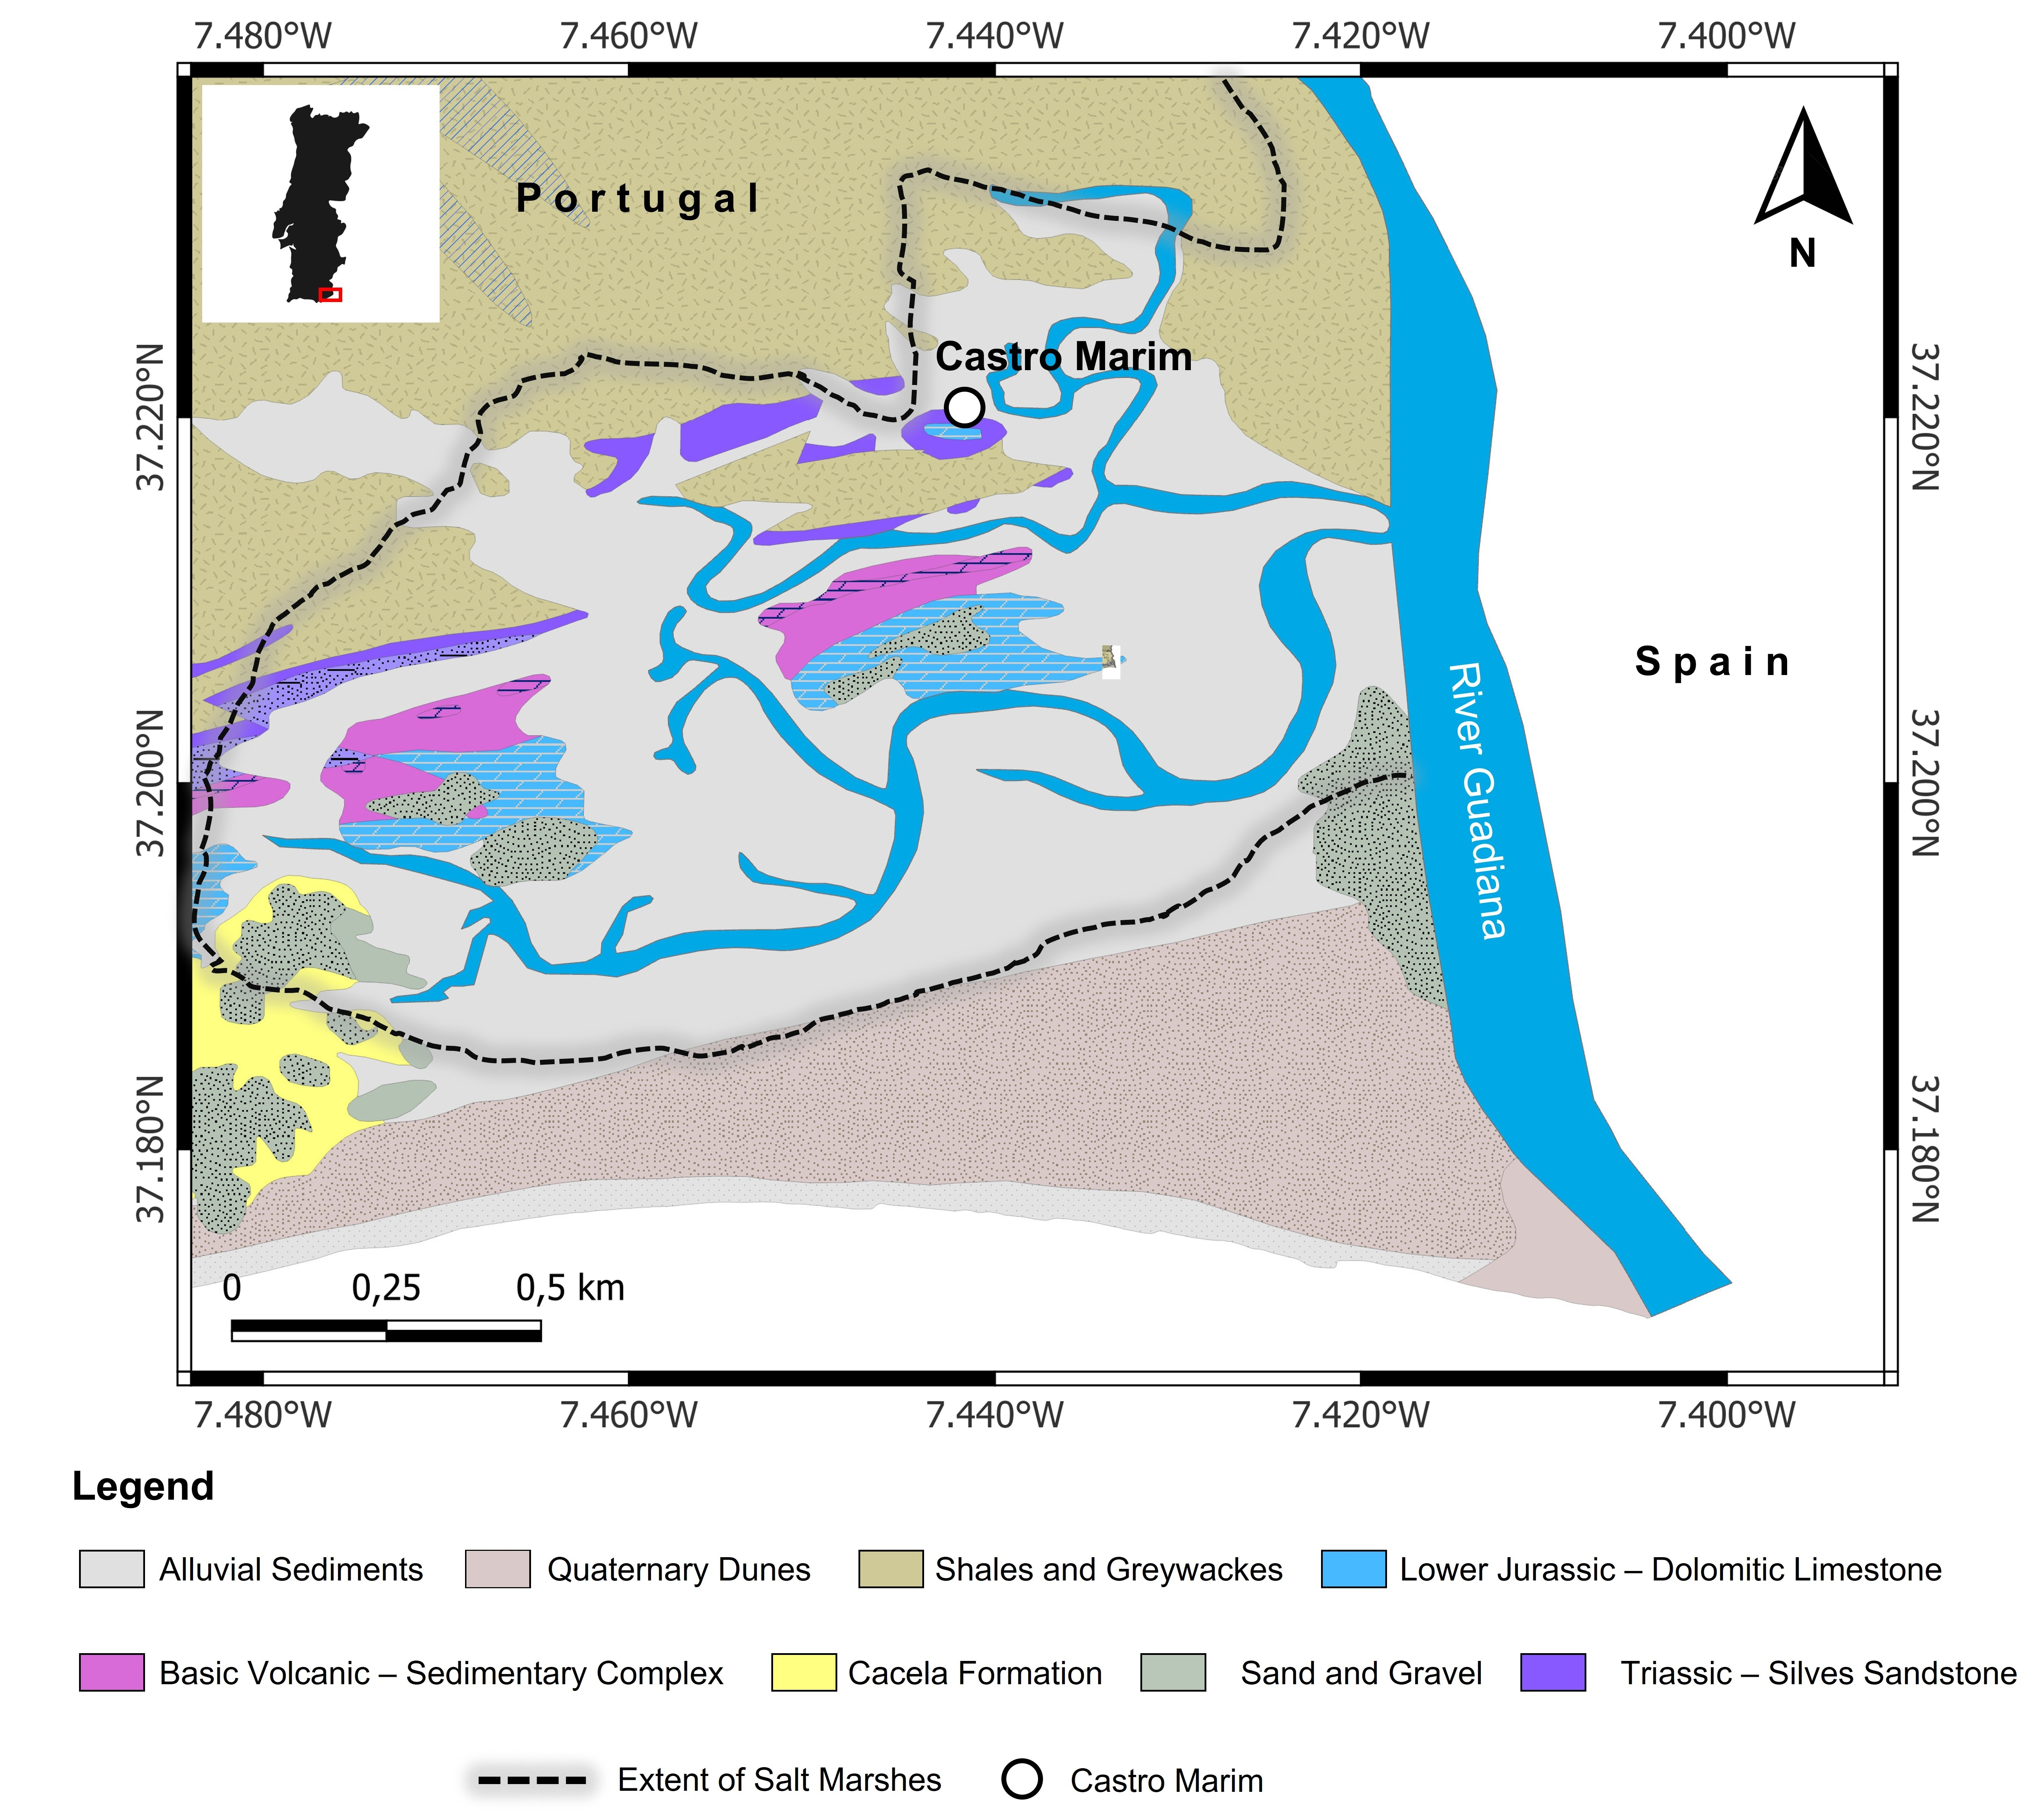
\includegraphics[width=0.98\textwidth]{C:/Users/rosha/Documents/R/Projects/castro_marim_phoenician/./images/castro_marim_map} \caption{Geological map of the region around Castro Marim on the banks of Guadiana River, Algarve Region of Portugal in EPSG 4326 projection. (Source: Directorate General of Mines and Geological Services - Carta de Geológica de Portugal).}\label{fig:castro-marim-loc}
\end{figure*}

\hypertarget{site-background}{%
\subsection{Site background}\label{site-background}}

Castro Marim is located on the Guadiana estuary (Fig. \ref{fig:castro-marim-loc}) as a portal to the metallogenic mineral-rich Baixo -- Alentejo region as well as to the fertile cultivable lands in the interior regions. The Iron Age settlement was located on an elevation with adequate natural defensive elements and overlooked vast swatches of land, which allowed domination of estuarine traffic and agricultural activities in its domain of influence. These conditions allowed trade and cultural networks between the indigenous communities and the Mediterranean communities to flourish. The earliest Iron Age occupation of the site is characterized by East-West orthogonal settlement architecture dating from the first half of 7\textsuperscript{th} century BCE, in the Orientalising period (\protect\hyperlink{ref-arruda_etal13}{Arruda et al., 2013}; \protect\hyperlink{ref-arruda96}{Arruda, 1996}).This earliest Iron Age occupation corresponds to Castro Marim´s phase II (1\textsuperscript{st} half of the 7\textsuperscript{th} century BCE), III (2\textsuperscript{nd} half of the 7\textsuperscript{th} century BCE) and IV (6\textsuperscript{th} century BCE). Phoenician imports and other evidence for human presence declined from the second half of the 6th century BCE till the first half of the 5\textsuperscript{th} century BCE (\protect\hyperlink{ref-arruda96}{Arruda, 1996}). Significant changes in material culture and restructuring of the settlement architecture with a Northeast -- Southwest orientation are observed from the second half of the 5\textsuperscript{th} century BCE (\protect\hyperlink{ref-arruda_etal13}{Arruda et al., 2013}, \protect\hyperlink{ref-arruda_etal06}{2006}; \protect\hyperlink{ref-arruda_freitas08}{Arruda and Freitas, 2008}). The earlier period's departure was marked by imports from Greek products -- specifically ceramics such as \emph{kilikes}, \emph{skyphoi}, and \emph{kantharoi} (\protect\hyperlink{ref-arruda_etal20}{Arruda et al., 2020}; \protect\hyperlink{ref-arruda97}{Arruda, 1997}). This resurgence put Castro Marim back in the main commercial circuits along the Iberian Peninsula's Atlantic coast till the 3\textsuperscript{rd} century BCE (\protect\hyperlink{ref-arruda_etal13}{Arruda et al., 2013}, \protect\hyperlink{ref-arruda_etal06}{2006}; \protect\hyperlink{ref-arruda00}{Arruda, 2000}; \protect\hyperlink{ref-sousa19}{Sousa, 2019}). The Phoenician -- Punic period is represented by archaeological phases III, IV, and V.

Being in a littoral zone made it possible to adopt a wide range of agricultural strategies and husbandry practices at Castro Marim. The presence of cereals (\emph{Hordeum} and \emph{Triticum}), grapes (\emph{Vitis vinifera/sylvestris}), pulses (\emph{Vicia} and \emph{Cicer}), and other cultivated species (\emph{Olea} and \emph{Coriandrum}), as well as the exploitation of wild woody plants (\emph{Pinus} and \emph{Arbutus} etc.) have been elucidated from the archaeological record (\protect\hyperlink{ref-queiroz_etal06}{Queiroz et al., 2006}). Animals recovered from the excavation (native to Portugal) include cattle (\emph{Bos taurus}), goat (\emph{Capra hircus}), sheep (\emph{Ovis aries}), pig (\emph{Sus scrofa/domesticus}), red deer (\emph{Cervus elaphus}), and rabbit (\emph{Oryctolagus cuniculus}) (\protect\hyperlink{ref-davis07}{Davis, 2007}). The arrival of chicken (\emph{Gallus domesticus}) has been documented, being introduced at least in the second half of 5\textsuperscript{th} century BCE (\protect\hyperlink{ref-davis07}{Davis, 2007}).

\hypertarget{environmental-settings}{%
\subsection{Environmental Settings}\label{environmental-settings}}



\begin{figure*}

{\centering 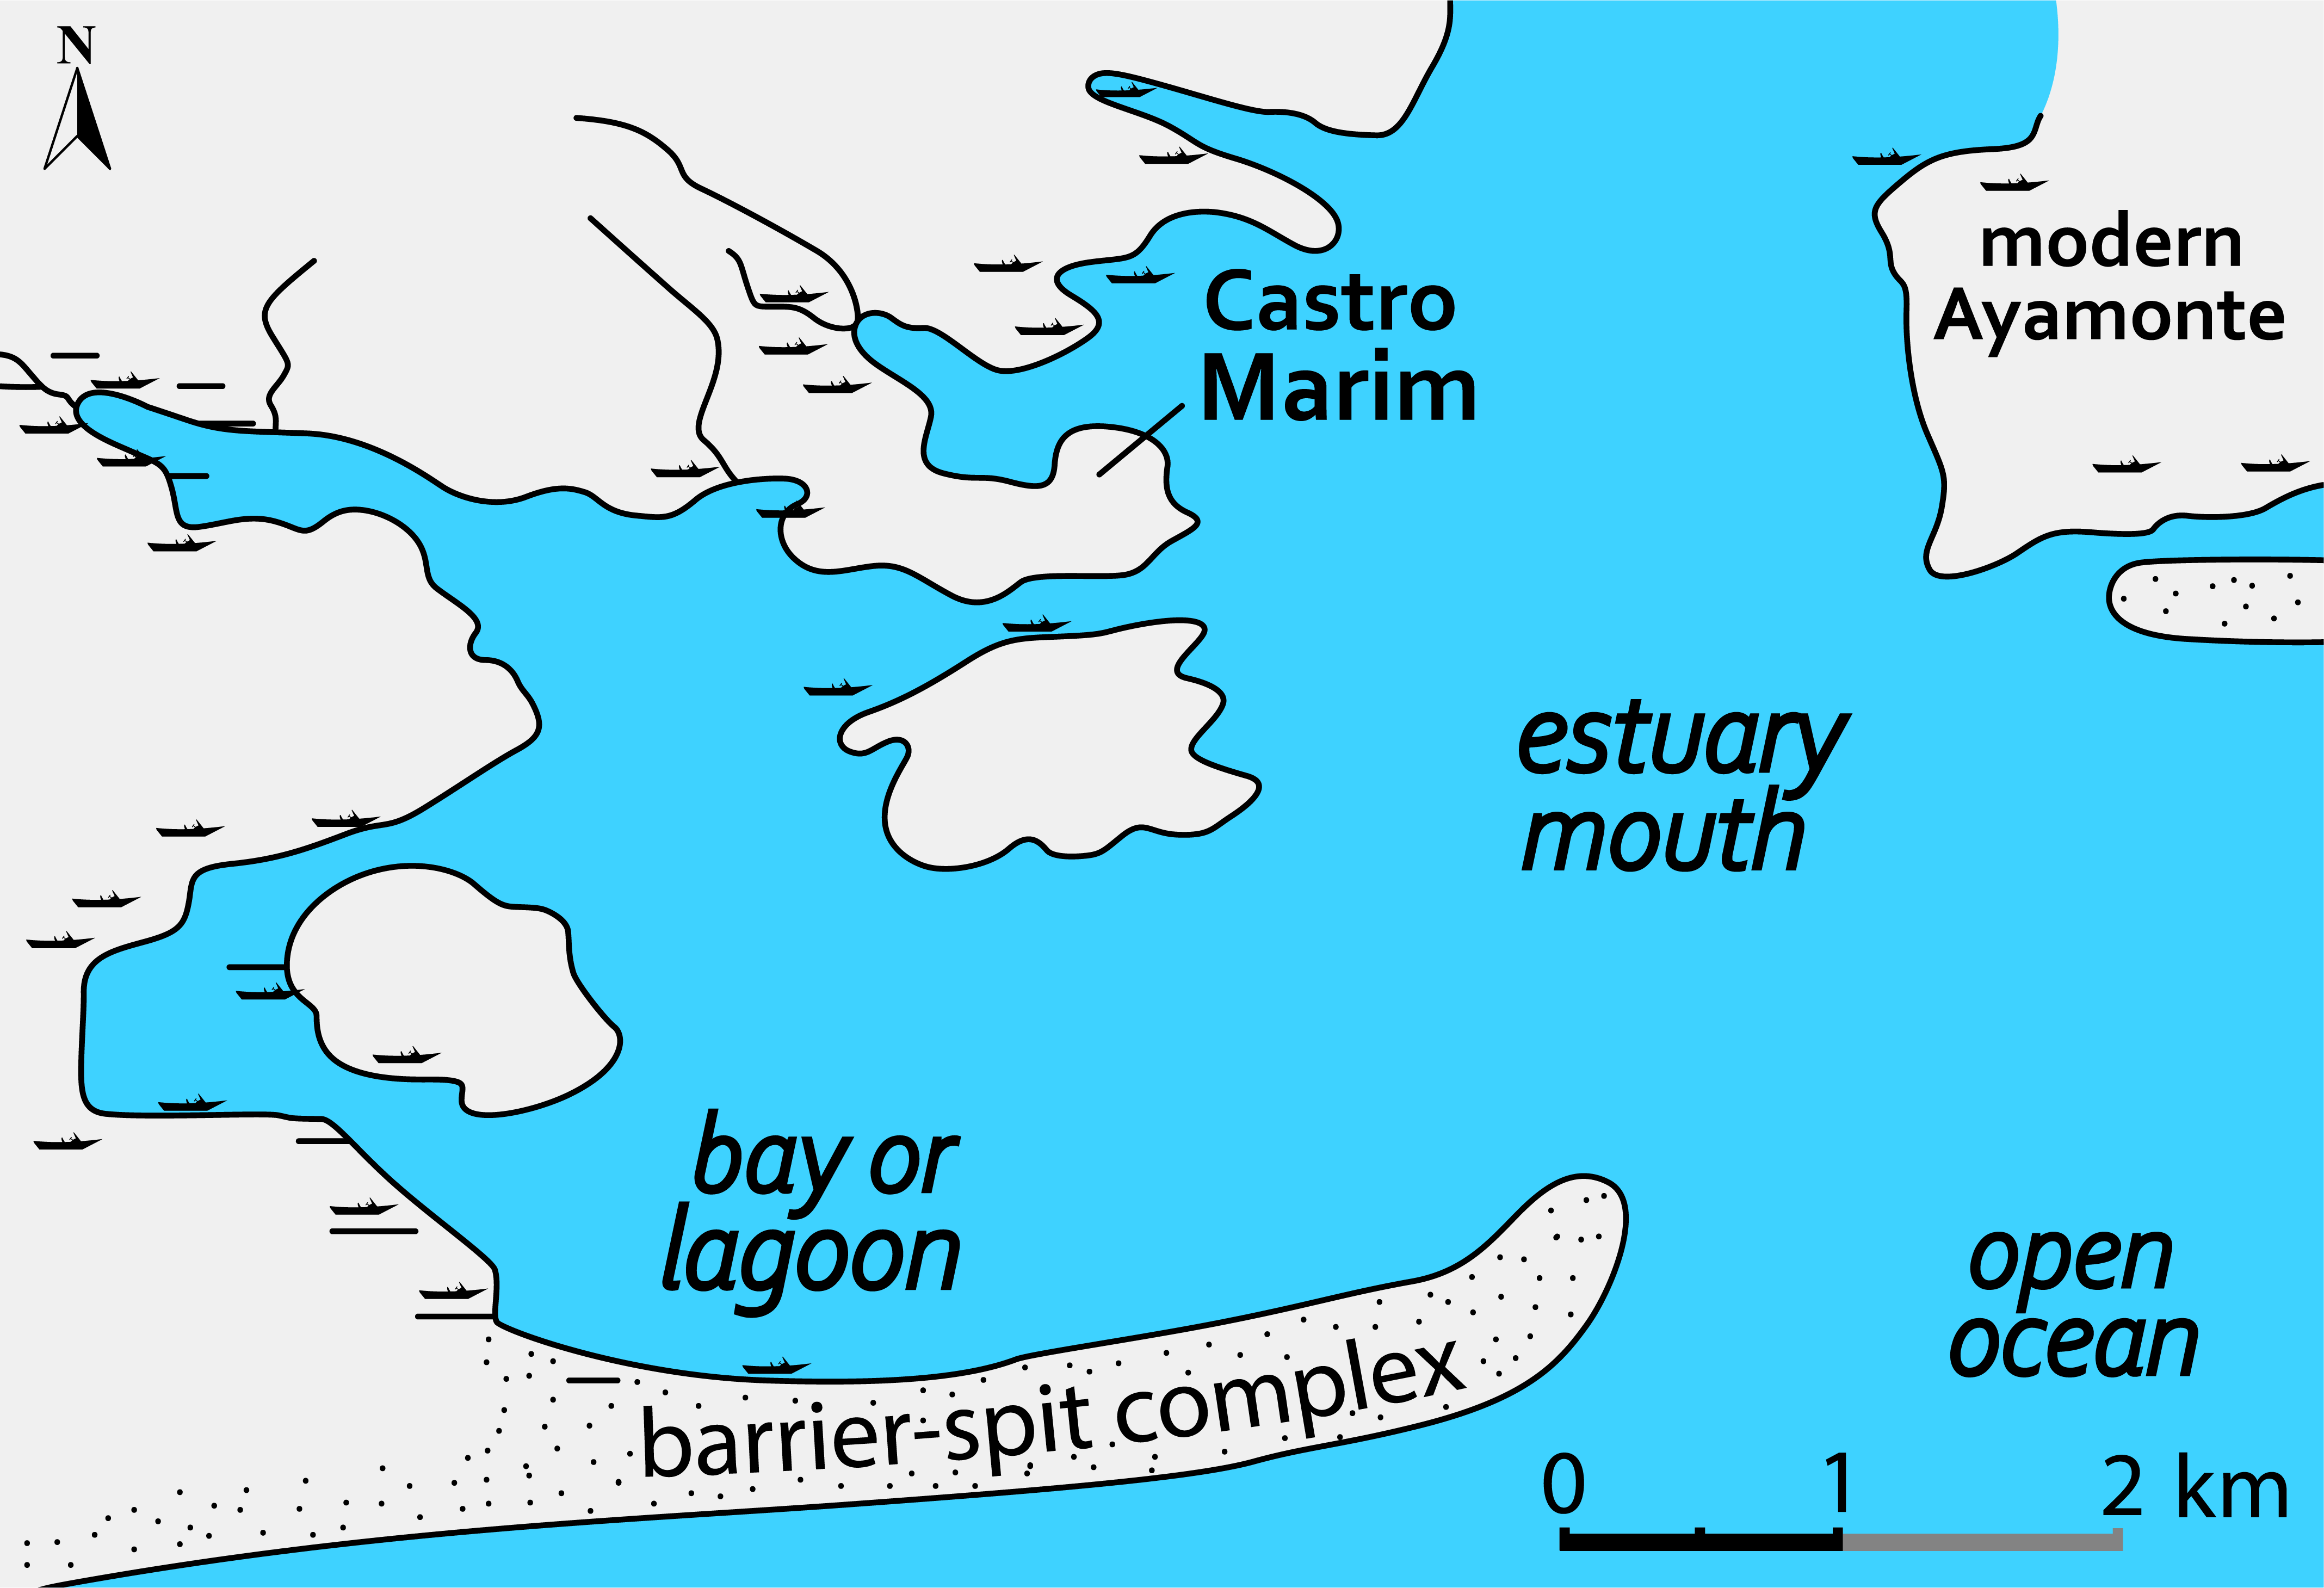
\includegraphics[width=0.60\textwidth]{C:/Users/rosha/Documents/R/Projects/castro_marim_phoenician/./images/castro_marim_pal} 

}

\caption{Reconstruction of the Guadiana estuary during the Phoenician period based on geophysical and lithological data (adapted from Wachsmann et al. (\protect\hyperlink{ref-wachsmann_etal09}{2009})).}\label{fig:castro-marim-pal}
\end{figure*}

Landscape surrounding during the Iron Age was quite different from what it is in modern times. Paleogeographic reconstruction based on geophysical and lithological data of the Guadiana estuary indicates muddy-bottom shallow estuarine setting at the mouth of the river during the Phoenician period, with the Iron Age settlement situated on a ridge projecting northward (Fig. \ref{fig:castro-marim-pal}) with a Pleistocene/mid-Holocene bedrock platform (\protect\hyperlink{ref-wachsmann_etal09}{Wachsmann et al., 2009}). After the arrival of Phoenicians (874 BCE), there was a decline in pinewood, \emph{Quercus} forest, and sclerophyllous thickets with an increase in scrub vegetation consisting of fire-adapted Cistaceae and Ericaceae (\protect\hyperlink{ref-fletcher_etal07}{Fletcher et al., 2007}). This is due to prevailing warm and dry climatic conditions corresponding to a more arid regime across southern Iberia (\protect\hyperlink{ref-jalut_etal00}{Jalut et al., 2000}; \protect\hyperlink{ref-magny_etal02}{Magny et al., 2002}).

\hypertarget{archaeobotanical-assessment}{%
\subsection{Archaeobotanical assessment}\label{archaeobotanical-assessment}}

The original archaeobotanical assessment was carried out by Queiroz et al. (\protect\hyperlink{ref-queiroz_etal06}{2006}). Cereals make up the most significant fraction of the carpological remains. The bulk of cereals is barley (\emph{Hordeum vulgare}) with a tiny fraction of wheat (\emph{Triticum durum/aestivum}). Pulses are mainly broad beans (\emph{Vicia faba}) and chickpeas (\emph{Cicer arietinum}), of which the former has been present in Portugal since prehistoric times, whereas the latter was appreciated as a luxury food in the Roman period from Asia. The presence of grape (\emph{Vitis vinifera/sylvestris}) pips and charred wood is typical, starting from the Phoenician period in Portugal. The presence of grape pips in Iron Age Castro Marim indicates exploitation of wild vines or cultivated non-local vines by the local population. The most exciting carpological remains are of coriander (\emph{Coriandrum sativum}) which is not native to Portugal and was supposed to be introduced during medieval times, making this the earliest coriander occurrence in Portugal. Charred pine, oak, ash, and poplar wood were recovered abundantly. The exploitation of wild woody plants for timber and fruits marks the Phoenician colonization of the Iberian peninsula. Due to unforeseen circumstances, these identified remains could not be accessed for isotope analyses. Previously unprocessed sediments were studied again to gain plant remains.

\hypertarget{zooarchaeological-assessment}{%
\subsection{Zooarchaeological assessment}\label{zooarchaeological-assessment}}

Ovicaprids (sheep and goats) followed by pigs and cattle dominate the Castro Marim mammal taxa (\protect\hyperlink{ref-davis07}{Davis, 2007}). Both sheep and goats were equally represented with negligible fluctuations throughout the Iron Age at Castro Marim. The wild species in the assemblage consisted mainly of red deer and rabbits. Both the species (red deer and rabbits) are present consistently in all the phases of the settlement. It is worth mentioning here that no morphometric distinction could be made between wild and domesticated pigs. There is a spike in the presence of bird remains in the later phases of the Iron Age (Phase IV - V), primarily due to the introduction of domesticated chicken. The presence of partridge, a common wild species of Iberia, is also noted. Unlike the chicken, partridge has never been domesticated. Ovicaprids and cattle were kept well into maturity indicating that they were prized more for their secondary purposes than their meat. Sheep and goats were kept for their milk and wool, usually slaughtered after they reach at least two years of age. Cattle were valued for their power to plow in the fields as well as to pull heavy loads. Also, they too, were a source of milk. Pigs, on the other hand, were slaughtered as juveniles as they were primarily reared for meat. Most of the red deer found were adults, suggesting a hunting preference of that period as a vital subsidiary source of meat. Chicken seems to be slaughtered at a young age, whereas the partridges at an adult age. The slaughter age indicates the domesticated status of chicken and wild status of partridge, respectively.

\hypertarget{methodological-approach}{%
\section{Methodological approach}\label{methodological-approach}}

\hypertarget{zooms-analysis-of-ovicaprids}{%
\subsection{ZooMS Analysis of Ovicaprids}\label{zooms-analysis-of-ovicaprids}}

Skeletal elements of goats and sheep are a common occurrence in archaeological contexts. A significant issue plaguing comparative husbandry studies between sheep and goats is the overlap of skeletal elements (\protect\hyperlink{ref-boessneck_etal64}{Boessneck et al., 1964}; \protect\hyperlink{ref-payne69}{Payne, 1969}; \protect\hyperlink{ref-schramm67}{Schramm, 1967}). Zooarchaeology through mass spectrometry applies peptide mass fingerprinting to identify archaeological remains (\protect\hyperlink{ref-buckley_etal09}{Buckley et al., 2009}). The main protein used for this is collagen, which is the most abundant protein in bone. Due to sequence differences in collagen of sheep and goat, ZooMS is able to differentiate between these two species, which is often not possible using standard morphological analysis (\protect\hyperlink{ref-buckley_etal10}{Buckley et al., 2010}).

\hypertarget{stable-isotope-analysis-of-plants-and-animals}{%
\subsection{Stable isotope analysis of plants and animals}\label{stable-isotope-analysis-of-plants-and-animals}}

Stable isotope (\(\delta ^{13}C\), and \(\delta ^{15}N\)) analyses of faunal bone collagen are valuable means of reconstructing foddering practices and other animal husbandry aspects (\protect\hyperlink{ref-price_etal17}{Price et al., 2017}). The variation in \(\delta ^{13}C\) of terrestrial organisms is determined by the primary producers' photosynthetic pathway, distinguished as C\textsubscript{3}, C\textsubscript{4}, and CAM plants (\protect\hyperlink{ref-deniro_epstein78}{DeNiro and Epstein, 1978}; \protect\hyperlink{ref-farquhar_etal89}{Farquhar et al., 1989}; \protect\hyperlink{ref-kohn10}{Kohn, 2010}; \protect\hyperlink{ref-tieszen91}{Tieszen, 1991}). Plant species are overwhelmingly C\textsubscript{3} in nature, including most cultivated plants such as barley, wheat, oats, and other wild edible plants (\protect\hyperlink{ref-fernandez-crespo_etal19}{Fernández-Crespo et al., 2019}). C\textsubscript{4} plants consist primarily of tropical grasses, millets, sugarcane, corn, and sorghum. C\textsubscript{4} plants thrive in warm and high-temperature environments and thus are restricted to coastal zones in regions with temperate climates (\protect\hyperlink{ref-leegood13}{Leegood, 2013}; \protect\hyperlink{ref-price_etal17}{Price et al., 2017}). The analysis of faunal bones can help in determining whether these animals ate C3 or C4 plants, as there is an enrichment in \(\delta ^{13}C\) between diet and consumers (5\text{\textperthousand} for herbivores and 0-2\text{\textperthousand} between trophic levels (\protect\hyperlink{ref-bocherens_drucker03}{Bocherens and Drucker, 2003})). \(\delta ^{13}C\) measurements are also helpful to differentiate between terrestrial C\textsubscript{3} and aquatic food sources (\protect\hyperlink{ref-froehle_etal10}{Froehle et al., 2010}; \protect\hyperlink{ref-kellner_schoeninger07}{Kellner and Schoeninger, 2007}).

\(\delta ^{15}N\) values indicate the trophic position (herbivore, omnivore, carnivore) of consumers in a food chain (\protect\hyperlink{ref-hedges_reynard07}{Hedges and Reynard, 2007}; \protect\hyperlink{ref-price_etal17}{Price et al., 2017}; \protect\hyperlink{ref-schoeninger85}{Schoeninger, 1985}), with an enrichment between diet and consumer of around 3-5\text{\textperthousand} (\protect\hyperlink{ref-hedges_reynard07}{Hedges and Reynard, 2007}; \protect\hyperlink{ref-schoeninger85}{Schoeninger, 1985}). \(\delta ^{15}N\) values can also be used to distinguish between terrestrial and marine diets (\protect\hyperlink{ref-deniro_epstein81}{Deniro and Epstein, 1981}; \protect\hyperlink{ref-webb_etal17a}{Webb et al., 2017}), and the consumption of manured, and unmanured crops (\protect\hyperlink{ref-bogaard_etal13}{Bogaard et al., 2013}; \protect\hyperlink{ref-deniro_epstein81}{Deniro and Epstein, 1981}; \protect\hyperlink{ref-fernandez-crespo_etal19}{Fernández-Crespo et al., 2019}; \protect\hyperlink{ref-fraser_etal13a}{Fraser et al., 2013}). \(\delta ^{34}S\) of bone collagen from terrestrial species is often measured along with \(\delta ^{13}C\) and \(\delta ^{15}N\) to identify consumption of marine foods (\protect\hyperlink{ref-nehlich_etal10}{Nehlich et al., 2010}).

The mean \(\delta ^{34}S\) value of terrestrial sources is assumed to be 0\text{\textperthousand} (\protect\hyperlink{ref-nehlich15}{Nehlich, 2015}). Inorganic sulphur enters the food web through plants from the weathered bedrock (in a complete terrestrial setting), precipitation (sea spray), and microbial activity due to flooding events (\protect\hyperlink{ref-nitsch_etal19}{Nitsch et al., 2019}). As the inorganic sulphur passes through the food web in the form of proteins, only a negligible fractionation occurs between diet and consumer (\protect\hyperlink{ref-hobson99}{Hobson, 1999}; \protect\hyperlink{ref-nehlich15}{Nehlich, 2015}). Thus, the \(\delta ^{34}S\) ratio of collagen closely reflects that of the native water source, bedrock, and soluble sulphur-bearing minerals.

There are two significant inputs that humans can manipulate to cultivate plants: water and nitrogen input, which can be investigated using stable isotopes. Variation in \(\delta ^{13}C\) values of plants is primarily due to water availability as any dry spells affect the movement of carbon dioxide through the stomata (\protect\hyperlink{ref-ferrio_etal07}{Ferrio et al., 2007}; \protect\hyperlink{ref-ferrio_etal05}{Ferrio et al., 2005}; \protect\hyperlink{ref-fiorentino_etal15}{Fiorentino et al., 2015}). The water status of crops can be artificially controlled by irrigation regimes, reflected in \(\delta ^{13}C\) values (\protect\hyperlink{ref-ferrio_etal05}{Ferrio et al., 2005}; \protect\hyperlink{ref-wallace_etal13}{Wallace et al., 2013}). \(\delta ^{13}C\) values measured in archaeological plants must be converted to carbon discrimination values to be compared with those of the modern crops grown under controlled watering regimes (\protect\hyperlink{ref-farquhar_etal89}{Farquhar et al., 1989}; \protect\hyperlink{ref-wallace_etal13}{Wallace et al., 2013}):

\[\Delta^{13}C = \frac{\delta ^{13}C_{air} - \delta ^{13}C_{plant}}{1+\delta ^{13}C_{plant}/1000}\] Another major factor, which affects the \(\delta ^{13}C\) measurements of plants, is the canopy effect, where forested areas are more depleted in the heavier \textsuperscript{13}C isotope compared to open areas (\protect\hyperlink{ref-bonafini_etal13}{Bonafini et al., 2013}). Thus, the \(\delta ^{13}C\) measurements of plants are the result of multiple factors and should be interpreted with caution.

One of the most ancient practices to increase soil fertility is by manuring with animal waste, as animal manure is much higher than endogenous soil in terms of nitrogen isotopic composition (\protect\hyperlink{ref-bogaard_etal13}{Bogaard et al., 2013}). Usually, the plants treated with manure exhibit higher \(\delta ^{15}N\) values (as much as 10\text{\textperthousand}) when compared to unfertilized plants (\protect\hyperlink{ref-bogaard_etal07}{Bogaard et al., 2007}; \protect\hyperlink{ref-fraser_etal11}{Fraser et al., 2011}). The \(\delta ^{13}C\) and \(\delta ^{15}N\) values themselves do not reveal the agricultural practices but reveal patterns when interpreted within a specific site.

\hypertarget{materials-and-methods}{%
\section{Materials and Methods}\label{materials-and-methods}}

\hypertarget{sample-selection}{%
\subsection{Sample Selection}\label{sample-selection}}

Fifty faunal bone samples (Table \ref{tab:table1}) from conclusively adult individuals as well as 9 charred plant macro-remains of \emph{Hordeum vulgare} subsp. \emph{vulgare}, \emph{Hordeum vulgare} subsp. \emph{nudum}, and \emph{Pinus} sp. each have been selected for this study. The sampled faunal bones represent the Phoenician -- Punic period of the settlement (phases III, IV, and V), whereas the charred plant macro -- remains are only from phase V due to the absence of plant remains from the older phases.

\hypertarget{archaeobotanical-analysis}{%
\subsection{Archaeobotanical Analysis}\label{archaeobotanical-analysis}}

200 grams of sediment from each stratigraphic layer of the excavation site was weighed and handpicked for plant macro remains (seeds/fruits and charcoal). The recovered remains were examined under a stereomicroscope and taxonomically identified (Table \ref{tab:table2}).

\hypertarget{bone-preservation-fourier-transform-infrared-spectroscopy}{%
\subsection{Bone Preservation: Fourier Transform Infrared Spectroscopy}\label{bone-preservation-fourier-transform-infrared-spectroscopy}}

500 -- 700 mg of bone was cut using a DREMEL\(\text{\textregistered}\) rotary drill with a diamond disc and cleaned of dirt, discoloration, and other foreign content with a dental burr. Compact bone was sampled over spongy bone. Bone fragments were slightly polished with fine sandpaper to obtain a flat surface (\protect\hyperlink{ref-hollund_etal13}{Hollund et al., 2013}). Infrared spectra were collected using a Bruker\(^\text{\textregistered}\) Alpha\(^\text{\texttrademark}\) Spectrometer with a single-reflection diamond crystal ATR module. Each spectrum was obtained by an accumulation of 128 scans with a spectral resolution of 4 cm\textsuperscript{-1}, from 2000 cm\textsuperscript{-1} to 375 cm\textsuperscript{-1}. Infrared Splitting Factor (IRSF) and relative carbonate content (C/P) were calculated using absorbance heights at 565 cm\textsuperscript{-1}, 590 cm\textsuperscript{-1}, 605 cm\textsuperscript{-1}, 1035 cm\textsuperscript{-1}, and 1415 cm\textsuperscript{-1} wavenumbers (\protect\hyperlink{ref-trueman_etal08}{Trueman et al., 2008}; \protect\hyperlink{ref-weiner_bar-yosef90}{Weiner and Bar-Yosef, 1990}; \protect\hyperlink{ref-wright_schwarcz96}{Wright and Schwarcz, 1996}).

\hypertarget{pretreatment-of-plant-macro-remains}{%
\subsection{Pretreatment of plant macro-remains}\label{pretreatment-of-plant-macro-remains}}

In carbonized plant macro-remains, barley grain samples consist of at least ten whole grains, and pine samples consist of shell fragment. Morphologically intact samples were chosen after examination under a stereomicroscope (7-45x magnification) and removing any visibly adhering foreign contaminant. An acid-base-acid (ABA) treatment was applied as a pre-treatment (\protect\hyperlink{ref-bogaard_etal13}{Bogaard et al., 2013}; \protect\hyperlink{ref-fraser_etal13a}{Fraser et al., 2013}). First, the samples were treated with 10 mL of 0.5 M HCl at 70 \(\text{\textdegree}\)C for 60 minutes (or until effervescing stops) and then rinsed with ultrapure water until a neutral pH was achieved. 10 mL of 0.1 NaOH solution was added to the samples at 70 \(\text{\textdegree}\)C for 60 minutes and then rinsed with ultrapure water to achieve a neutral pH. Finally, the samples were treated with 0.5 M HCl at 70 \(\text{\textdegree}\)C for 30-60 minutes, followed by three rinses with ultrapure water and subsequent freeze-drying.

\hypertarget{collagen-extraction}{%
\subsection{Collagen Extraction}\label{collagen-extraction}}

The modified Longin (\protect\hyperlink{ref-longin71}{1971}) method was used to extract collagen from faunal bones pieces previously analysed with FTIR by demineralization (\protect\hyperlink{ref-richards_hedges99}{Richards and Hedges, 1999}). Approximately 600 mg of bone sample was demineralized using 0.5 M HCl at 4 \(\text{\textdegree}\)C for a fortnight with daily vortex and an acid change after 7 days. Repeated rinses with ultrapure water to reach neutral pH were performed, and the demineralized bones were subjected to an overnight treatment in 0.125 M NaOH at room temperature to remove fulvic and humic acid contamination. The samples were then rinsed repeatedly with ultrapure water to achieve neutrality and gelatinized in 0.01 M HCl at 70 \(\text{\textdegree}\)C for 48 hours. The impurities were separated by filtering the collagen-containing liquid fraction using Ezee -- Filter\(^\text{\texttrademark}\) filters (Elkay\(^\text{\textregistered}\) Laboratory Products). The solubilized collagen was frozen and subsequently lyophilized for 48 hours.

\hypertarget{zooms-analysis}{%
\subsection{ZooMS analysis}\label{zooms-analysis}}

A small subsample of the extracted collagen was placed into a microfuge tube and 100 \(\mu\)L 50mM ammonium bicarbonate (Ambic) was added to the samples. The samples were digested overnight using 1 \(\mu\)L of 0.5 \(\mu\)g/\(\mu\)L porcine trypsin (Promega\(^\text{\textregistered}\), UK) at 37 \(\text{\textdegree}\)C and the digestion was stopped by the addition of trifluoroacetic acid (TFA) at a concentration of 0.5--1 \% of the total solution. The samples were desalted using C18 zip-tips (\protect\hyperlink{ref-vandoorn_etal11}{van Doorn et al., 2011}) and eluted using 100 \(\mu\)L of 50\% acetonitrile (ACN)/0.1 \% TFA (v/v). The zip-tipped samples were spotted in triplicate onto a MTP384 Bruker ground steel MALDI target plate; 1 \(\mu\)L of sample was pipetted onto each sample spot and then mixed with 1 \(\mu\)L of \(\alpha\)-cyano-4-hydroxycinnamic acid matrix solution (1 \% in 50 \% acetonitrile / 0.1 \% trifluoroacetic acid (v/v/v)).

The samples were analysed on a Bruker\(^\text{\textregistered}\) Ultraflex III\(^\text{\texttrademark}\) MALDI-ToF mass spectrometer. The resulting MS spectra were analysed using mMass (\protect\hyperlink{ref-strohalm_etal10}{Strohalm et al., 2010}) an Open Source mass spectrometry interpretation tool. The three spectra for each sample were averaged and the averaged spectrum was cropped between 800 and 3000 m/z and peak picking was carried out using a signal to noise ratio of 6. The resulting spectra were compared to a publicly available ZooMS database.

\hypertarget{stable-carbon-and-nitrogen-isotope-analysis}{%
\subsection{Stable carbon and nitrogen isotope analysis}\label{stable-carbon-and-nitrogen-isotope-analysis}}

An amount of 0.5 - 0.7 mg of freeze-dried collagen powder/barley grain samples were weighed in tin capsules and combusted in an elemental analyzer (EA) with oxygen (Flash 2000 HT\(^\text{\texttrademark}\), Thermo Fisher Scientific\(^\text{\textregistered}\), Bremen, Germany) using pure helium as carrier gas. Isotopic ratios were obtained on a Delta V Advantage Continuous Flow\(^\text{\texttrademark}\) -- Isotope Ratio Mass Spectrometer (Thermo Fisher Scientific\(^\text{\textregistered}\), Bremen, Germany). The raw machine output was normalised by a three-point calibration using international standard reference materials (SRM), namely IAEA-CH-6 (sucrose, \(\delta ^{13}C\) = -- 10.499\text{\textperthousand}), IAEA-600 (caffeine, \(\delta ^{13}C\) = -- 27.771\text{\textperthousand}; \(\delta ^{15}N\) = + 1\text{\textperthousand}), and IAEA-N-2 (ammonium sulphate, \(\delta ^{15}N\) = + 20.3\text{\textperthousand}) and in-house standard L-Alanine (\(\delta ^{13}C\) = -- 18.5\text{\textperthousand}; \(\delta ^{15}N\) = + 1.1\text{\textperthousand}). The standards were regularly (after eleven analyses) included in the analytical routine to correct for instrumental drifts. The isotope values are expressed in per mil (\text{\textperthousand}) relative to VPDB (Vienna Pee-Dee Belemnite) for carbon and AIR (Ambient Inhalable Reservoir) for nitrogen. In order to correct for charring effect in plant remains, 0.11\text{\textperthousand} and 0.31\text{\textperthousand} were subtracted from their \(\delta ^{13}C\) and \(\delta ^{15}N\) values, respectively (\protect\hyperlink{ref-nitsch_etal15}{Nitsch et al., 2015}). The fluctuations in \(\delta ^{13}C\) of the atmospheric CO\textsubscript{2} throughout the Holocene were considered while interpreting the stable carbon isotope ratios. The \(\delta ^{13}C\) of atmospheric CO\textsubscript{2} during the period in the study was approximated using the AIRCO\textsubscript{2}\_LOESS system, and then this value was used to compute the \(\delta ^{13}C\) discrimination of plants independent of the source CO\textsubscript{2} (\protect\hyperlink{ref-farquhar_etal82}{Farquhar et al., 1982}; \protect\hyperlink{ref-ferrio_etal05}{Ferrio et al., 2005}).

\hypertarget{stable-sulphur-isotope-analysis}{%
\subsection{Stable sulphur isotope analysis}\label{stable-sulphur-isotope-analysis}}

The collagen samples were combusted with additional V\textsubscript{2}O\textsubscript{5} and an oxygen pulse (IsoPrime\(^\text{\texttrademark}\) Mass spectrometer, Elementar Analysensysteme GmbH\(^\text{\textregistered}\), Langenselbold, Germany). Calibration of \(\delta ^{34}S\) values was performed using international inorganic standards for stable sulphur isotope analysis: NBS127 (+20.3\text{\textperthousand}) and IAEA S1 (-0.3\text{\textperthousand}). B2155 protein (+6.96 ± 0.04\text{\textperthousand}) was used as an internal quality control standard. Stable sulphur isotope values are reported in parts per thousand relative to Vienna-Canyon Diablo Troilite (VCDT).

\hypertarget{statistical-analysis}{%
\subsection{Statistical Analysis}\label{statistical-analysis}}

The obtained data were subjected to statistical analysis using R programming language (\protect\hyperlink{ref-rcoreteam20}{R Core Team, 2020}; \protect\hyperlink{ref-wickham16}{Wickham, 2016}). Initially, means and standard deviations were calculated per species. Z-scores were calculated to detect the presence of outliers. Deviance from normal distribution was assessed using the Shapiro-Wilks test. F-tests were first used to check for significant equal variance, and subsequently, unpaired Student's t-tests were used for two-sample comparison since all the datasets were normally distributed.

\hypertarget{results-and-discussion}{%
\section{Results and Discussion}\label{results-and-discussion}}

\hypertarget{bone-preservation}{%
\subsection{Bone Preservation}\label{bone-preservation}}

\begingroup\fontsize{7.5}{9.5}\selectfont

\begin{longtable}[t]{cccccc}
\caption{\label{tab:table1}Collagen yield and FT-IR results (IRSF and C/P) of selected faunal bone samples.}\\
\toprule
Sample ID & Species & Phase & Collagen yield (\%) & IRSF & C/P\\
\midrule
\endfirsthead
\caption[]{\label{tab:table1}Collagen yield and FT-IR results (IRSF and C/P) of selected faunal bone samples. \textit{(continued)}}\\
\toprule
Sample ID & Species & Phase & Collagen yield (\%) & IRSF & C/P\\
\midrule
\endhead

\endfoot
\bottomrule
\endlastfoot
CMOF779 & Pluvialis squatarola & III & 2.5 & 2.43 & 0.26\\
CMOF777 & Rissa tridactyla & V & 3.9 & 3.37 & 0.40\\
CMOF756 & Alectoris rufa & IV & 8.8 & 2.53 & 0.33\\
CMOF737 & Alectoris rufa & V & 6.3 & 2.79 & 0.23\\
CMOF710 & Gallus domesticus & V & 4.5 & 2.63 & 0.25\\
CMOF774 & Gallus domesticus & V & 10.5 & 2.87 & 0.35\\
CMOF750 & Gallus domesticus & V & 6.0 & 2.65 & 0.41\\
CMOF751 & Gallus domesticus & V & 31.1 & 3.28 & 0.31\\
CMOF772 & Gallus domesticus & V & 3.1 & 2.91 & 0.22\\
CMOF743 & Gallus domesticus & V & 4.5 & 2.74 & 0.22\\
CMOF746 & Gallus domesticus & V & 24.7 & 2.54 & 0.28\\
CMOF744 & Gallus domesticus & V & 6.5 & 2.37 & 0.41\\
CMOF731 & Gallus domesticus & V & 10.4 & 2.54 & 0.30\\
CMOF730 & Gallus domesticus & V & 15.8 & 2.48 & 0.30\\
CMOF709 & Gallus domesticus & V & 29.1 & 3.12 & 0.40\\
CMOF745 & Gallus domesticus & V & 4.5 & 2.83 & 0.30\\
CMOF158 & Sus scrofa & III & 5.1 & 2.78 & 0.40\\
CMOF439 & Sus scrofa & IV & 6.6 & 3.24 & 0.25\\
CMOF354 & Sus scrofa & IV & 41.4 & 2.75 & 0.28\\
CMOF253 & Sus scrofa & IV & 16.2 & 2.65 & 0.37\\
CMOF338 & Sus scrofa & V & 6.0 & 2.61 & 0.22\\
CMOF466 & Sus scrofa & V & 19.8 & 2.59 & 0.23\\
CMOF323 & Sus scrofa & V & 2.6 & 3.33 & 0.29\\
CMOF435 & Bos taurus & III & 10.9 & 2.98 & 0.21\\
CMOF370 & Bos taurus & III & 41.6 & 2.78 & 0.38\\
CMOF402 & Bos taurus & III & 12.3 & 2.45 & 0.36\\
CMOF201 & Bos taurus & IV & 29.1 & 2.96 & 0.37\\
CMOF480 & Bos taurus & IV & 10.8 & 2.56 & 0.40\\
CMOF147 & Bos taurus & IV & 19.8 & 2.62 & 0.40\\
CMOF468 & Bos taurus & V & 22.9 & 3.27 & 0.30\\
CMOF393 & Bos taurus & V & 36.2 & 2.39 & 0.42\\
CMOF94 & Bos taurus & V & 34.0 & 3.14 & 0.37\\
CMOF397 & Capra hircus & III & 13.3 & 2.87 & 0.43\\
CMOF181 & Capra hircus & III & 24.6 & 2.97 & 0.26\\
CMOF420 & Capra hircus & IV & 19.8 & 2.66 & 0.21\\
CMOF673 & Capra hircus & IV & 20.9 & 2.40 & 0.37\\
CMOF660 & Capra hircus & IV & 4.0 & 2.60 & 0.28\\
CMOF14 & Capra hircus & V & 7.9 & 2.59 & 0.34\\
CMOF394 & Capra hircus & V & 21.4 & 2.47 & 0.24\\
CMOF424 & Ovis aries & III & 45.7 & 2.48 & 0.21\\
CMOF374 & Ovis aries & III & 15.6 & 2.41 & 0.41\\
CMOF419 & Ovis aries & IV & 9.6 & 3.14 & 0.41\\
CMOF463 & Ovis aries & IV & 5.3 & 2.93 & 0.20\\
CMOF656 & Ovis aries & IV & 49.1 & 2.50 & 0.38\\
CMOF260 & Ovis aries & IV & 6.8 & 2.61 & 0.34\\
CMOF691 & Ovis aries & V & 6.8 & 2.79 & 0.42\\
CMOF477 & Ovis aries & V & 10.8 & 2.59 & 0.22\\
CMOF303 & Ovis aries & V & 17.8 & 2.39 & 0.28\\
CMOF230 & Oryctolagus cuniculus & III & 8.4 & 3.01 & 0.37\\
CMOF254 & Oryctolagus cuniculus & IV & 7.2 & 3.01 & 0.32\\
CMOF99 & Oryctolagus cuniculus & V & 6.5 & 3.12 & 0.20\\
CMOF457 & Oryctolagus cuniculus & V & 4.9 & 2.81 & 0.23\\
CMOF353 & Oryctolagus cuniculus & V & 23.1 & 3.31 & 0.20\\
CMOF334 & Oryctolagus cuniculus & V & 11.0 & 3.26 & 0.31\\
CMOF324 & Oryctolagus cuniculus & V & 7.7 & 2.79 & 0.42\\
CMOF388 & Cervus elaphus & III & 6.7 & 2.59 & 0.29\\
CMOF373 & Cervus elaphus & III & 6.3 & 2.60 & 0.39\\
CMOF677 & Cervus elaphus & IV & 6.2 & 2.51 & 0.34\\
CMOF467 & Cervus elaphus & V & 15.5 & 2.64 & 0.36\\
CMOF508 & Cervus elaphus & V & 3.0 & 2.50 & 0.23\\
CMOF643 & Cervus elaphus & V & 8.4 & 2.69 & 0.28\\
CMOF504 & Cervus elaphus & V & 10.9 & 2.69 & 0.36\\*
\end{longtable}
\endgroup{}

\hypertarget{fourier-transform---infrared-spectroscopy}{%
\subsubsection{Fourier Transform - Infrared Spectroscopy}\label{fourier-transform---infrared-spectroscopy}}

The IRSF index values (Table \ref{tab:table1}) are in a range of 2.37 - 3.37 (accepted range is 2.96 - 4.04), and the C/P index values are in the range of 0.2-0.428 (accepted range is 0.054 - 0.47), which fall well within the accepted range for crystallinity and carbonate content of well-preserved archaeological bones (\protect\hyperlink{ref-hollund_etal13}{Hollund et al., 2013}; \protect\hyperlink{ref-lebon_etal16}{Lebon et al., 2016}).

\hypertarget{collagen-quality}{%
\subsubsection{Collagen Quality}\label{collagen-quality}}

Collagen yields range between 2.5\% to 49.1\% (Table \ref{tab:table1}). Collagen extraction was considered successful for all the bone samples, based on published criteria, with carbon content between 15.3\% and 47.0\% (\protect\hyperlink{ref-ambrose90}{Ambrose, 1990}), nitrogen content between 5.5\% and 17.3\% (\protect\hyperlink{ref-ambrose90}{Ambrose, 1990}), C/N values between 2.9 and 3.6 (\protect\hyperlink{ref-deniro85}{DeNiro, 1985}), C/S values between 300\% and 900\% (\protect\hyperlink{ref-nehlich_richards09}{Nehlich and Richards, 2009}), and collagen yields greater than 1\% (\protect\hyperlink{ref-vanklinken99}{Klinken, 1999}). The extracted bone collagen samples exhibit C/N values ranged between 3.1 and 3.5 and C/S values between 225.9 and 688.4. Carbon and nitrogen amounts range from 20.3\% to 50.0\% and 7.3\% and 18.1\% respectively. All the faunal samples exhibited collagen quality parameters indicative of good preservation.

\hypertarget{zooms-results}{%
\subsection{ZooMS Results}\label{zooms-results}}

Sheep and goat samples were successfully distinguished on the basis of ZooMS. The identified sample entries are in bold format (Table \ref{tab:table4}).

\hypertarget{botanical-remains}{%
\subsection{Botanical Remains}\label{botanical-remains}}

\begin{table}[!h]

\caption{\label{tab:table2}Recovered plant remains from archaeological sediments.}
\centering
\fontsize{7.5}{9.5}\selectfont
\begin{tabular}[t]{>{}lcc}
\toprule
Species & Quantity & Phase\\
\midrule
\em{Hordeum vulgare} & 1300 & V\\
\em{Triticum aestivum/durum} & 4 & V\\
\em{Apium graveolens} & 1 & V\\
\em{Pinus pinea} & 2 & V\\
\em{Brassica nigra} & 3 & V\\
\em{Pisum sativum} & 1 & V\\
\em{Galeopsis tetrahit} & 1 & V\\
\em{Vicia faba} & 2 & V\\
\bottomrule
\end{tabular}
\end{table}

No botanical remains could be recovered from the soil samples of phases I -- IV. The bulk of the recovered remains are from phase V representing the most mature chronological period of the occupation. Barley (\emph{Hordeum vulgare}) is the dominant taxon in the botanical record (Table \ref{tab:table2}). \emph{Hordeum vulgare} var. \emph{nudum} and \emph{Hordeum vulgare} subsp. \emph{vulgare} (Fig. \ref{fig:castro-archbot-assemblage} \textbf{(f)} and \textbf{(g)}, respectively) are the two cultivars that constitute the barley fraction with equal abundance. Wheat (\emph{Triticum aestivum/durum}) is the second most abundant taxon after barley. Large-scale cereal cultivation has been observed in sites located in river valleys near the South Iberian sea coast (including, Castillo de Doña Blanca in Guadalquivir Valley and El Villar in Guadalhorce Valley) (\protect\hyperlink{ref-semmler92}{Semmler, 1992}, \protect\hyperlink{ref-semmler90}{1990}), two sites which are located in similar geographical settings to Castro Marim). Cereal cultivation seems to be a significant activity, implying that cereals were the principal source of carbohydrates for both humans and animals. The greater presence of barley compared to wheat can be a strategy of `minimum returns on investment' against dry climatic conditions exploiting the fact that barley has a higher tolerance to drier conditions than wheat (\protect\hyperlink{ref-riehl09}{Riehl, 2009}). Two taxa of pulses have been noted, namely, peas (\emph{Pisum sativum}) and broad bean (\emph{Vicia faba}) (Fig. \ref{fig:castro-archbot-assemblage} \textbf{(d)} and \textbf{(i)} respectively). Pulses serve as a rich source of proteins and act as an alternative to animal-sourced protein for humans. The combined cultivation of pulses with cereals helps to maintain adequate soil nitrogen levels, leading to sustainable and diverse production. The presence of black mustard (\emph{Brassica nigra}) (Fig. \ref{fig:castro-archbot-assemblage} \textbf{(a)}) has been recorded. Black mustard is a common species along the rocky Mediterranean coasts and has long found its place as a culinary taste enhancer (\protect\hyperlink{ref-dixon06}{Dixon, 2006}). Like many members of \emph{Brassica}, black mustard was also used as a source of oil (\protect\hyperlink{ref-pena-chocarro_etal19}{Peña-Chocarro et al., 2019}).



\begin{figure*}
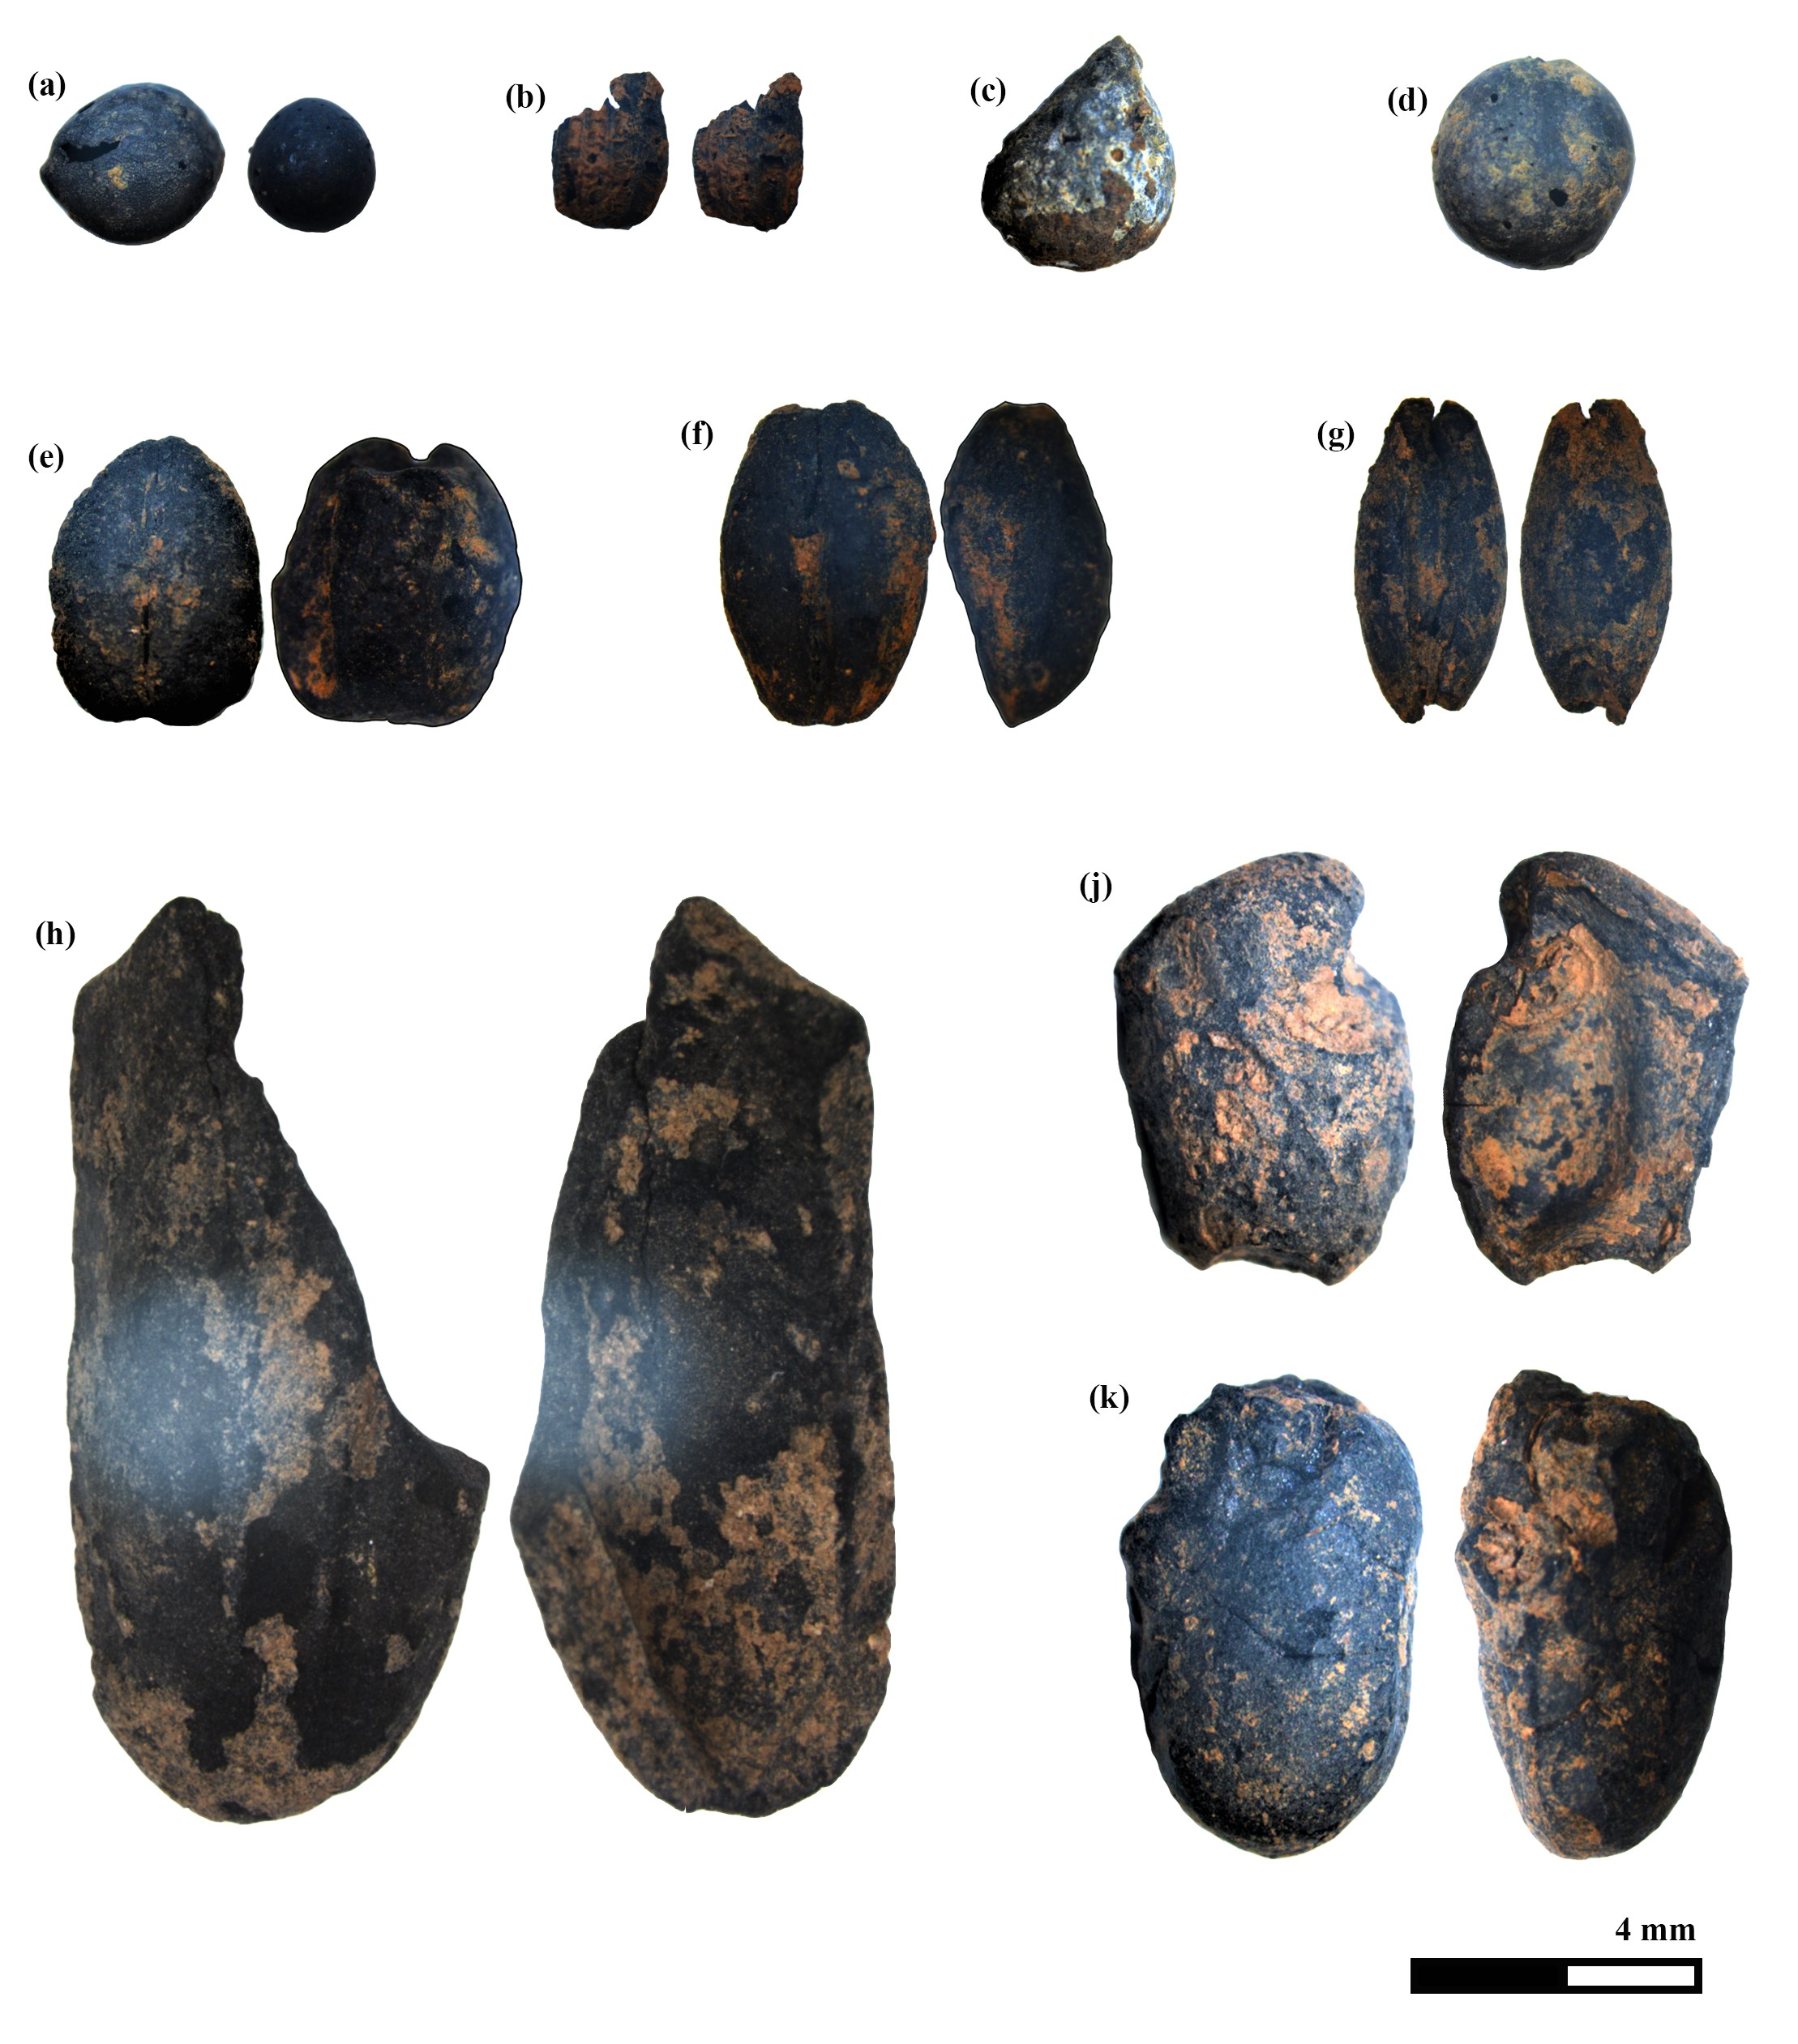
\includegraphics[width=0.98\textwidth]{C:/Users/rosha/Documents/R/Projects/castro_marim_phoenician/./images/castro_bot_assemblage} \caption{Charred plant remains of settlement phase V from Castro Marim; \textbf{(a)} \emph{Brassica nigra}; \textbf{(b)} \emph{Apium graveolens}; \textbf{(c)} \emph{Galeopsis tetrahit}; \textbf{(d)} \emph{Pisum sativum}; \textbf{(e)} \emph{Triticum aestivum/durum}; \textbf{(f)} \emph{Hordeum vulgare} var. \emph{nudum}; \textbf{(g)} \emph{Hordeum vulgare} subsp. \emph{vulgare}; \textbf{(h)} \emph{Pinus pinea}; \textbf{(i)} \emph{Vicia faba}}\label{fig:castro-archbot-assemblage}
\end{figure*}

A fragment of a charred fruit has been attributed to \emph{Apium} taxon, suspected to be a seed of celery (\emph{Apium graveolens}) (Fig. \ref{fig:castro-archbot-assemblage} \textbf{(b)}). This attribution is done due to the presence of five slender longitudinal ridges on the surface of the fruit (\protect\hyperlink{ref-wilson16}{Wilson, 2016}).This species is native to the coastal Mediterranean region, considered to be its center of origin. The recorded use of celery as a vegetable in Europe is only from the 1600s, originating in Italy, gradually spreading westwards in the subsequent centuries (\protect\hyperlink{ref-tobyn_etal11}{Tobyn et al., 2011}). The consumption of celery as a vegetable started in the Mediterranean region only around the 16\textsuperscript{th} century CE. In the Phoenician - Punic period, it could have been either cultivated or foraged as a medicinal herb rather than a food plant (\protect\hyperlink{ref-sturtevant86}{Sturtevant, 1886}). Shells of pine nuts (\emph{Pinus} sp.) (Fig. \ref{fig:castro-archbot-assemblage} \textbf{(h)}) are suspected to be from the species \emph{Pinus pinea}, commonly known as Mediterranean stone pine. Pine nut consumption has been documented in Portugal since the Palaeolithic period (\protect\hyperlink{ref-gale_carruthers00}{Gale and Carruthers, 2000}). The stone pine nuts are high in protein and fat with low carbohydrates (\protect\hyperlink{ref-haws04}{Haws, 2004}). The nuts are a valuable source of nutrition and could have been stored during low cultivated food production periods.





\begin{table*}

\caption{\label{tab:table3}\(\delta ^{13}C\) and \(\delta ^{15}N\) values of the charred plant macro-remains.}
\centering
\resizebox{\linewidth}{!}{
\fontsize{7.5}{9.5}\selectfont
\begin{tabu} to \linewidth {>{\centering}X>{}c>{\raggedright}X>{\raggedright}X>{\raggedright}X>{\raggedright}X>{\raggedright}X>{\raggedright}X>{\centering}X}
\toprule
Sample ID & Species & \% C & \% N & $\delta^{13}C$  (\text{\textperthousand}) & $\delta^{15}N$ 
 (\text{\textperthousand}) & $\delta^{13}C_{cr}^{*}$ 
 (\text{\textperthousand}) & $\delta^{15}N_{cr}^{*}$ 
 (\text{\textperthousand}) & $\Delta^{13}C$ 
 (\text{\textperthousand})\\
\midrule
CMHV1 & \em{Hordeum vulgare {\normalfont subsp.} vulgare} & 37.7 & 2.1 & -22.1 & 9.6 & -22.2 & 9.3 & 16.1\\
CMHV2 & \em{Hordeum vulgare {\normalfont subsp.} vulgare} & 49.7 & 2.8 & -22.6 & 9.4 & -22.7 & 9.1 & 16.6\\
CMHV3 & \em{Hordeum vulgare {\normalfont subsp.} vulgare} & 50.0 & 2.2 & -24.7 & 9.1 & -24.8 & 8.8 & 18.8\\
CMHN1 & \em{Hordeum vulgare {\normalfont var.} nudum} & 49.1 & 3.6 & -23.0 & 8.9 & -23.1 & 8.6 & 17.0\\
CMHN2 & \em{Hordeum vulgare {\normalfont var.} nudum} & 49.5 & 3.9 & -23.2 & 8.4 & -23.3 & 8.1 & 17.2\\
CMHN3 & \em{Hordeum vulgare {\normalfont var.} nudum} & 47.6 & 2.6 & -23.1 & 9.8 & -23.2 & 9.5 & 17.1\\
CMPP1 & \em{Pinus pinea} & 58.8 & 0.7 & -25.5 & 11.4 & -25.6 & 11.1 & 19.6\\
CMPP2 & \em{Pinus pinea} & 48.3 & 0.8 & -24.7 & 11.3 & -24.8 & 11.0 & 18.8\\
CMPP3 & \em{Pinus pinea} & 56.7 & 0.6 & -25.4 & 13.8 & -25.5 & 13.5 & 19.5\\
\bottomrule
\multicolumn{9}{l}{\rule{0pt}{1em}\textsuperscript{*} \(\delta ^{13}C\) and \(\delta ^{15}N\) values corrected for charring effect.}\\
\end{tabu}}
\end{table*}

\hypertarget{water-and-nutrient-nitrogen-availability-for-vegetation}{%
\subsection{Water and nutrient nitrogen availability for vegetation}\label{water-and-nutrient-nitrogen-availability-for-vegetation}}

Table \ref{tab:table3} shows the results of stable isotope ratios of the two barley cultivars and stone pine. In the case of barley, the isotope ratios fall within the established predicted ranges obtained from experimentally charred modern cereals (\protect\hyperlink{ref-fraser_etal13a}{Fraser et al., 2013}). Since the isotope ratios of the stone pine are similar to that of barley, they are considered consistent. The \(\delta ^{13}C\) values of all the plants are within the range expected for C\textsubscript{3} plants with mean values of -23.2 ± 1.4\text{\textperthousand}, -23.2 ± 0.1\text{\textperthousand}, and -25.3 ± 0.4\text{\textperthousand} for \emph{Hordeum vulgare} var. \emph{nudum}, \emph{Hordeum vulgare} subsp. \emph{vulgare}, and \emph{Pinus pinea} respectively. Though the plants are located close to the coast (Fig. \ref{fig:castro-marim-loc}), the source of carbon is from the atmosphere (\protect\hyperlink{ref-cloern_etal02}{Cloern et al., 2002}), and thus the values are similar to terrestrial plants. The \(\delta ^{13}C\) means of both barley cultivars show no statistically significant difference (t-statistic: -0.04, degrees of freedom: 4, \emph{p}-value: 0.97). The \(\Delta ^{13}C\) values (Figure \ref{fig:iso-hord-plots} \textbf{(a)}) show barley cultivated in poor to moderate watering conditions, which would indicate that the plants have been dependent on natural precipitation with little or no artificial irrigation in an arid climatic regime (\protect\hyperlink{ref-fernandez-crespo_etal19}{Fernández-Crespo et al., 2019}; \protect\hyperlink{ref-fletcher_etal07}{Fletcher et al., 2007}).



\begin{figure}
\centering
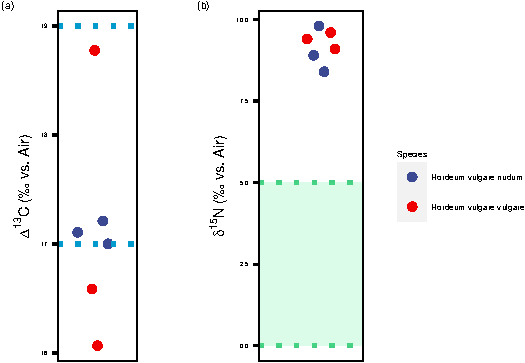
\includegraphics{castro_main_body_files/figure-latex/iso-hord-plots-1.pdf}
\caption{\label{fig:iso-hord-plots}\textbf{(a).} Beeswarm plot showing \(\Delta ^{13}C\) values of barley cultivars where the area between the blue dashed lines represents `moderately-watered' condition with the `well-watered' condition being above the top blue line and `poorly-watered' condition being below the lower blue line, based on the study of modern crops in varying watering conditions (\protect\hyperlink{ref-wallace_etal13}{Wallace et al., 2013}). \textbf{(b).} Beeswarm plot showing the manuring status of barley cultivars with green shaded region representing 1 SD range of estimated wild herbivore forage value (calculated from subtraction 4 \text{\textperthousand} from red deer \(\delta ^{15}N\) mean ± 1 SD range).}
\end{figure}

The plants analysed all exhibit high \(\delta ^{15}N\) mean values of 9.1 ± 0.3\text{\textperthousand}, 8.7 ± 0.7\text{\textperthousand} and 11.9 ± 1.4\text{\textperthousand} for \emph{Hordeum vulgare} var. \emph{nudum}, \emph{Hordeum vulgare} subsp. \emph{vulgare}, and \emph{Pinus pinea} respectively. There is no significant difference (t-statistic: 0.77, degrees of freedom: 4, \emph{p}-value: 0.49) between the two barley cultivars, but Pinus pinea yields higher \(\delta ^{15}N\) values. The \(\delta ^{15}N\) mean values of the plants in salt marshes are higher when compared to completely inland sites (\protect\hyperlink{ref-cloern_etal02}{Cloern et al., 2002}). The \(\delta ^{15}N\) isotope ratios are elevated, as the coastal/saline soils are enriched in nutrient nitrogen because of nitrate sea-spray, nitrification, denitrification, and ammonium absorption (\protect\hyperlink{ref-ambrose91}{Ambrose, 1991}; \protect\hyperlink{ref-heaton87}{Heaton, 1987}; \protect\hyperlink{ref-virginia_delwiche82}{Virginia and Delwiche, 1982}). The stone pine samples exhibit higher mean values than the barley cultivars despite the possibility that the latter could be subjected to manuring regimes (Figure \ref{fig:iso-hord-plots} \textbf{(b)}). This indicates that the barley was cultivated in locations farther away from the coastline than the stone pine and explains the poor to moderate watering conditions despite Castro Marim being close to Guadiana estuary. Because the settlement was located on a narrow strip of land surrounded by water (Figure \ref{fig:castro-marim-pal}), the lack of space to grow crops must have been the primary reason for growing the barley away from the coast. Thus, any effects of manure on \(\delta ^{15}N\) isotope ratios of barley are masked by the increase caused by the proximity to the coast/salt marsh.

\begingroup\fontsize{7.5}{9.5}\selectfont

\begin{longtable}[t]{c>{}cccccccccc}
\caption{\label{tab:table4}Carbon, nitrogen, and sulphur isotope composition of the fauna.}\\
\toprule
Sample ID & Species & \% C & \% N & \% S & C:N & C:S & N:S & $\delta^{13}C (\text{\textperthousand})$ & $\delta^{15}N (\text{\textperthousand})$ & $\delta^{34}S (\text{\textperthousand})$\\
\midrule
\endfirsthead
\caption[]{\label{tab:table4}Carbon, nitrogen, and sulphur isotope composition of the fauna. \textit{(continued)}}\\
\toprule
Sample ID & Species & \% C & \% N & \% S & C:N & C:S & N:S & $\delta^{13}C (\text{\textperthousand})$ & $\delta^{15}N (\text{\textperthousand})$ & $\delta^{34}S (\text{\textperthousand})$\\
\midrule
\endhead

\endfoot
\bottomrule
\multicolumn{11}{l}{\rule{0pt}{1em}\textit{Note: }}\\
\multicolumn{11}{l}{\rule{0pt}{1em}The ovicaprid samples which were identified as goats and sheep are in bold.}\\
\endlastfoot
CMOF779 & \em{Pluvialis squatarola} & 40.8 & 14.8 & 0.3 & 3.2 & 375.9 & 81.6 & -14.9 & 10.3 & 9.5\\
CMOF777 & \em{Rissa tridactyla} & 40.9 & 15.1 & 0.3 & 3.2 & 376.9 & 109.7 & -15.5 & 13.9 & 15.8\\
CMOF756 & \em{Alectoris rufa} & 41.0 & 15.1 & 0.3 & 3.2 & 438.1 & 53.3 & -20.6 & 5.8 & 13.9\\
CMOF737 & \em{Alectoris rufa} & 40.6 & 14.9 & 0.3 & 3.2 & 416.8 & 49.0 & -20.0 & 5.6 & 13.9\\
CMOF710 & \em{Gallus domesticus} & 40.5 & 14.7 & 0.3 & 3.2 & 415.9 & 81.5 & -18.9 & 9.3 & 16.2\\
CMOF774 & \em{Gallus domesticus} & 40.7 & 14.9 & 0.2 & 3.2 & 452.9 & 74.4 & -20.2 & 7.8 & 15.1\\
CMOF750 & \em{Gallus domesticus} & 40.6 & 15.1 & 0.2 & 3.1 & 451.9 & 94.8 & -18.2 & 9.9 & 13.5\\
CMOF751 & \em{Gallus domesticus} & 40.6 & 14.8 & 0.2 & 3.2 & 515.8 & 106.5 & -18.1 & 9.8 & 14.9\\
CMOF772 & \em{Gallus domesticus} & 40.7 & 14.9 & 0.2 & 3.2 & 452.8 & 91.1 & -18.5 & 9.6 & 14.9\\
CMOF743 & \em{Gallus domesticus} & 41.1 & 15.0 & 0.2 & 3.2 & 498.4 & 100.2 & -18.1 & 9.6 & 12.5\\
CMOF746 & \em{Gallus domesticus} & 42.4 & 15.8 & 0.2 & 3.1 & 514.6 & 100.4 & -17.3 & 9.6 & 12.2\\
CMOF744 & \em{Gallus domesticus} & 43.4 & 16.0 & 0.3 & 3.2 & 429.3 & 80.1 & -17.5 & 9.5 & 14.7\\
CMOF731 & \em{Gallus domesticus} & 42.8 & 15.6 & 0.3 & 3.2 & 393.6 & 86.0 & -19.3 & 10.9 & 16.2\\
CMOF730 & \em{Gallus domesticus} & 50.0 & 18.1 & 0.2 & 3.2 & 606.3 & 115.5 & -19.6 & 11.1 & 14.1\\
CMOF709 & \em{Gallus domesticus} & 42.8 & 15.7 & 0.2 & 3.2 & 544.0 & 119.8 & -18.7 & 11.0 & 14.6\\
CMOF745 & \em{Gallus domesticus} & 41.0 & 15.3 & 0.2 & 3.1 & 476.1 & 95.2 & -18.2 & 9.6 & 15.2\\
CMOF158 & \em{Sus scrofa} & 41.0 & 15.2 & 0.2 & 3.2 & 521.0 & 119.5 & -19.3 & 11.0 & 14.6\\
CMOF439 & \em{Sus scrofa} & 21.7 & 8.0 & -- & 3.2 & -- & -- & -19.8 & 8.8 & --\\
CMOF354 & \em{Sus scrofa} & 40.9 & 15.3 & 0.2 & 3.1 & 496.0 & 133.8 & -18.0 & 12.9 & 11.4\\
CMOF253 & \em{Sus scrofa} & 40.3 & 15.0 & 0.2 & 3.1 & 489.3 & 76.3 & -19.6 & 7.3 & 11.9\\
CMOF338 & \em{Sus scrofa} & 40.8 & 15.0 & -- & 3.2 & -- & -- & -20.3 & 8.5 & --\\
CMOF466 & \em{Sus scrofa} & 40.8 & 15.0 & 0.2 & 3.2 & 544.1 & 100.4 & -20.1 & 8.8 & 14.4\\
CMOF323 & \em{Sus scrofa} & 40.4 & 14.9 & -- & 3.2 & -- & -- & -20.3 & 7.3 & --\\
CMOF435 & \em{Bos taurus} & 41.1 & 14.9 & 0.2 & 3.2 & 477.5 & 88.9 & -20.2 & 8.9 & 10.3\\
CMOF370 & \em{Bos taurus} & 39.8 & 14.6 & 0.2 & 3.2 & 443.1 & 66.7 & -21.2 & 7.0 & 15.2\\
CMOF402 & \em{Bos taurus} & 41.8 & 15.8 & -- & 3.1 & -- & -- & -19.0 & 7.6 & --\\
CMOF201 & \em{Bos taurus} & 41.9 & 15.6 & 0.2 & 3.1 & 558.6 & 69.4 & -21.4 & 6.1 & 8.3\\
CMOF480 & \em{Bos taurus} & 39.1 & 14.4 & 0.2 & 3.2 & 580.6 & 52.5 & -21.7 & 4.1 & 15.3\\
CMOF147 & \em{Bos taurus} & 43.0 & 16.2 & -- & 3.1 & -- & -- & -20.0 & 7.2 & --\\
CMOF468 & \em{Bos taurus} & 40.9 & 15.5 & 0.2 & 3.1 & 642.4 & 122.8 & -21.6 & 9.1 & 11.6\\
CMOF393 & \em{Bos taurus} & 42.1 & 15.3 & -- & 3.2 & -- & -- & -20.3 & 3.9 & --\\
CMOF94 & \em{Bos taurus} & 36.7 & 13.9 & 0.2 & 3.1 & 490.4 & 58.0 & -20.9 & 5.1 & 7.8\\
\cellcolor{white}{\textcolor{black}{\textbf{CMOF397}}} & \em{\cellcolor{white}{\textcolor{black}{\textbf{Capra hircus}}}} & \cellcolor{white}{\textcolor{black}{\textbf{38.7}}} & \cellcolor{white}{\textcolor{black}{\textbf{14.2}}} & \cellcolor{white}{\textcolor{black}{\textbf{0.2}}} & \cellcolor{white}{\textcolor{black}{\textbf{3.2}}} & \cellcolor{white}{\textcolor{black}{\textbf{688.4}}} & \cellcolor{white}{\textcolor{black}{\textbf{64.5}}} & \cellcolor{white}{\textcolor{black}{\textbf{-19.8}}} & \cellcolor{white}{\textcolor{black}{\textbf{4.2}}} & \cellcolor{white}{\textcolor{black}{\textbf{10.9}}}\\
\cellcolor{white}{\textcolor{black}{\textbf{CMOF181}}} & \em{\cellcolor{white}{\textcolor{black}{\textbf{Capra hircus}}}} & \cellcolor{white}{\textcolor{black}{\textbf{41.3}}} & \cellcolor{white}{\textcolor{black}{\textbf{15.3}}} & \cellcolor{white}{\textcolor{black}{\textbf{0.2}}} & \cellcolor{white}{\textcolor{black}{\textbf{3.2}}} & \cellcolor{white}{\textcolor{black}{\textbf{580.4}}} & \cellcolor{white}{\textcolor{black}{\textbf{59.5}}} & \cellcolor{white}{\textcolor{black}{\textbf{-19.8}}} & \cellcolor{white}{\textcolor{black}{\textbf{4.9}}} & \cellcolor{white}{\textcolor{black}{\textbf{12.6}}}\\
\cellcolor{white}{\textcolor{black}{\textbf{CMOF420}}} & \em{\cellcolor{white}{\textcolor{black}{\textbf{Capra hircus}}}} & \cellcolor{white}{\textcolor{black}{\textbf{40.7}}} & \cellcolor{white}{\textcolor{black}{\textbf{15.1}}} & \cellcolor{white}{\textcolor{black}{\textbf{0.2}}} & \cellcolor{white}{\textcolor{black}{\textbf{3.2}}} & \cellcolor{white}{\textcolor{black}{\textbf{494.3}}} & \cellcolor{white}{\textcolor{black}{\textbf{59.4}}} & \cellcolor{white}{\textcolor{black}{\textbf{-19.3}}} & \cellcolor{white}{\textcolor{black}{\textbf{5.7}}} & \cellcolor{white}{\textcolor{black}{\textbf{13.6}}}\\
\cellcolor{white}{\textcolor{black}{\textbf{CMOF673}}} & \em{\cellcolor{white}{\textcolor{black}{\textbf{Capra hircus}}}} & \cellcolor{white}{\textcolor{black}{\textbf{20.3}}} & \cellcolor{white}{\textcolor{black}{\textbf{7.3}}} & \cellcolor{white}{\textcolor{black}{\textbf{0.2}}} & \cellcolor{white}{\textcolor{black}{\textbf{3.3}}} & \cellcolor{white}{\textcolor{black}{\textbf{225.9}}} & \cellcolor{white}{\textcolor{black}{\textbf{51.9}}} & \cellcolor{white}{\textcolor{black}{\textbf{-19.2}}} & \cellcolor{white}{\textcolor{black}{\textbf{5.4}}} & \cellcolor{white}{\textcolor{black}{\textbf{14.8}}}\\
\cellcolor{white}{\textcolor{black}{\textbf{CMOF660}}} & \em{\cellcolor{white}{\textcolor{black}{\textbf{Capra hircus}}}} & \cellcolor{white}{\textcolor{black}{\textbf{42.3}}} & \cellcolor{white}{\textcolor{black}{\textbf{15.6}}} & \cellcolor{white}{\textcolor{black}{\textbf{0.2}}} & \cellcolor{white}{\textcolor{black}{\textbf{3.2}}} & \cellcolor{white}{\textcolor{black}{\textbf{564.3}}} & \cellcolor{white}{\textcolor{black}{\textbf{48.5}}} & \cellcolor{white}{\textcolor{black}{\textbf{-19.8}}} & \cellcolor{white}{\textcolor{black}{\textbf{4.2}}} & \cellcolor{white}{\textcolor{black}{\textbf{12.8}}}\\
\cellcolor{white}{\textcolor{black}{\textbf{CMOF14}}} & \em{\cellcolor{white}{\textcolor{black}{\textbf{Capra hircus}}}} & \cellcolor{white}{\textcolor{black}{\textbf{36.6}}} & \cellcolor{white}{\textcolor{black}{\textbf{13.1}}} & \cellcolor{white}{\textcolor{black}{\textbf{--}}} & \cellcolor{white}{\textcolor{black}{\textbf{3.3}}} & \cellcolor{white}{\textcolor{black}{\textbf{--}}} & \cellcolor{white}{\textcolor{black}{\textbf{--}}} & \cellcolor{white}{\textcolor{black}{\textbf{-20.3}}} & \cellcolor{white}{\textcolor{black}{\textbf{3.9}}} & \cellcolor{white}{\textcolor{black}{\textbf{--}}}\\
\cellcolor{white}{\textcolor{black}{\textbf{CMOF394}}} & \em{\cellcolor{white}{\textcolor{black}{\textbf{Capra hircus}}}} & \cellcolor{white}{\textcolor{black}{\textbf{27.2}}} & \cellcolor{white}{\textcolor{black}{\textbf{10.0}}} & \cellcolor{white}{\textcolor{black}{\textbf{0.2}}} & \cellcolor{white}{\textcolor{black}{\textbf{3.2}}} & \cellcolor{white}{\textcolor{black}{\textbf{426.9}}} & \cellcolor{white}{\textcolor{black}{\textbf{85.7}}} & \cellcolor{white}{\textcolor{black}{\textbf{-19.6}}} & \cellcolor{white}{\textcolor{black}{\textbf{6.4}}} & \cellcolor{white}{\textcolor{black}{\textbf{9.2}}}\\
\cellcolor{white}{\textcolor{black}{\textbf{CMOF424}}} & \em{\cellcolor{white}{\textcolor{black}{\textbf{Ovis aries}}}} & \cellcolor{white}{\textcolor{black}{\textbf{40.6}}} & \cellcolor{white}{\textcolor{black}{\textbf{14.8}}} & \cellcolor{white}{\textcolor{black}{\textbf{0.2}}} & \cellcolor{white}{\textcolor{black}{\textbf{3.2}}} & \cellcolor{white}{\textcolor{black}{\textbf{493.1}}} & \cellcolor{white}{\textcolor{black}{\textbf{73.3}}} & \cellcolor{white}{\textcolor{black}{\textbf{-20.7}}} & \cellcolor{white}{\textcolor{black}{\textbf{7.0}}} & \cellcolor{white}{\textcolor{black}{\textbf{7.7}}}\\
\cellcolor{white}{\textcolor{black}{\textbf{CMOF374}}} & \em{\cellcolor{white}{\textcolor{black}{\textbf{Ovis aries}}}} & \cellcolor{white}{\textcolor{black}{\textbf{41.1}}} & \cellcolor{white}{\textcolor{black}{\textbf{15.3}}} & \cellcolor{white}{\textcolor{black}{\textbf{0.3}}} & \cellcolor{white}{\textcolor{black}{\textbf{3.1}}} & \cellcolor{white}{\textcolor{black}{\textbf{406.0}}} & \cellcolor{white}{\textcolor{black}{\textbf{68.4}}} & \cellcolor{white}{\textcolor{black}{\textbf{-17.3}}} & \cellcolor{white}{\textcolor{black}{\textbf{8.1}}} & \cellcolor{white}{\textcolor{black}{\textbf{13.4}}}\\
\cellcolor{white}{\textcolor{black}{\textbf{CMOF419}}} & \em{\cellcolor{white}{\textcolor{black}{\textbf{Ovis aries}}}} & \cellcolor{white}{\textcolor{black}{\textbf{36.8}}} & \cellcolor{white}{\textcolor{black}{\textbf{13.5}}} & \cellcolor{white}{\textcolor{black}{\textbf{0.2}}} & \cellcolor{white}{\textcolor{black}{\textbf{3.2}}} & \cellcolor{white}{\textcolor{black}{\textbf{516.5}}} & \cellcolor{white}{\textcolor{black}{\textbf{67.1}}} & \cellcolor{white}{\textcolor{black}{\textbf{-20.8}}} & \cellcolor{white}{\textcolor{black}{\textbf{5.6}}} & \cellcolor{white}{\textcolor{black}{\textbf{7.0}}}\\
\cellcolor{white}{\textcolor{black}{\textbf{CMOF463}}} & \em{\cellcolor{white}{\textcolor{black}{\textbf{Ovis aries}}}} & \cellcolor{white}{\textcolor{black}{\textbf{40.7}}} & \cellcolor{white}{\textcolor{black}{\textbf{15.3}}} & \cellcolor{white}{\textcolor{black}{\textbf{0.2}}} & \cellcolor{white}{\textcolor{black}{\textbf{3.1}}} & \cellcolor{white}{\textcolor{black}{\textbf{543.5}}} & \cellcolor{white}{\textcolor{black}{\textbf{86.6}}} & \cellcolor{white}{\textcolor{black}{\textbf{-20.8}}} & \cellcolor{white}{\textcolor{black}{\textbf{7.6}}} & \cellcolor{white}{\textcolor{black}{\textbf{15.9}}}\\
\cellcolor{white}{\textcolor{black}{\textbf{CMOF656}}} & \em{\cellcolor{white}{\textcolor{black}{\textbf{Ovis aries}}}} & \cellcolor{white}{\textcolor{black}{\textbf{40.9}}} & \cellcolor{white}{\textcolor{black}{\textbf{15.2}}} & \cellcolor{white}{\textcolor{black}{\textbf{0.2}}} & \cellcolor{white}{\textcolor{black}{\textbf{3.1}}} & \cellcolor{white}{\textcolor{black}{\textbf{574.2}}} & \cellcolor{white}{\textcolor{black}{\textbf{46.8}}} & \cellcolor{white}{\textcolor{black}{\textbf{-19.8}}} & \cellcolor{white}{\textcolor{black}{\textbf{3.9}}} & \cellcolor{white}{\textcolor{black}{\textbf{17.3}}}\\
\cellcolor{white}{\textcolor{black}{\textbf{CMOF260}}} & \em{\cellcolor{white}{\textcolor{black}{\textbf{Ovis aries}}}} & \cellcolor{white}{\textcolor{black}{\textbf{42.5}}} & \cellcolor{white}{\textcolor{black}{\textbf{15.9}}} & \cellcolor{white}{\textcolor{black}{\textbf{--}}} & \cellcolor{white}{\textcolor{black}{\textbf{3.1}}} & \cellcolor{white}{\textcolor{black}{\textbf{--}}} & \cellcolor{white}{\textcolor{black}{\textbf{--}}} & \cellcolor{white}{\textcolor{black}{\textbf{-19.8}}} & \cellcolor{white}{\textcolor{black}{\textbf{5.9}}} & \cellcolor{white}{\textcolor{black}{\textbf{--}}}\\
\cellcolor{white}{\textcolor{black}{\textbf{CMOF691}}} & \em{\cellcolor{white}{\textcolor{black}{\textbf{Ovis aries}}}} & \cellcolor{white}{\textcolor{black}{\textbf{40.9}}} & \cellcolor{white}{\textcolor{black}{\textbf{15.4}}} & \cellcolor{white}{\textcolor{black}{\textbf{0.2}}} & \cellcolor{white}{\textcolor{black}{\textbf{3.1}}} & \cellcolor{white}{\textcolor{black}{\textbf{545.9}}} & \cellcolor{white}{\textcolor{black}{\textbf{106.4}}} & \cellcolor{white}{\textcolor{black}{\textbf{-20.7}}} & \cellcolor{white}{\textcolor{black}{\textbf{9.3}}} & \cellcolor{white}{\textcolor{black}{\textbf{12.4}}}\\
\cellcolor{white}{\textcolor{black}{\textbf{CMOF477}}} & \em{\cellcolor{white}{\textcolor{black}{\textbf{Ovis aries}}}} & \cellcolor{white}{\textcolor{black}{\textbf{43.9}}} & \cellcolor{white}{\textcolor{black}{\textbf{15.6}}} & \cellcolor{white}{\textcolor{black}{\textbf{0.2}}} & \cellcolor{white}{\textcolor{black}{\textbf{3.3}}} & \cellcolor{white}{\textcolor{black}{\textbf{558.3}}} & \cellcolor{white}{\textcolor{black}{\textbf{61.0}}} & \cellcolor{white}{\textcolor{black}{\textbf{-19.5}}} & \cellcolor{white}{\textcolor{black}{\textbf{5.6}}} & \cellcolor{white}{\textcolor{black}{\textbf{8.8}}}\\
\cellcolor{white}{\textcolor{black}{\textbf{CMOF303}}} & \em{\cellcolor{white}{\textcolor{black}{\textbf{Ovis aries}}}} & \cellcolor{white}{\textcolor{black}{\textbf{42.1}}} & \cellcolor{white}{\textcolor{black}{\textbf{15.7}}} & \cellcolor{white}{\textcolor{black}{\textbf{0.2}}} & \cellcolor{white}{\textcolor{black}{\textbf{3.1}}} & \cellcolor{white}{\textcolor{black}{\textbf{562.5}}} & \cellcolor{white}{\textcolor{black}{\textbf{80.0}}} & \cellcolor{white}{\textcolor{black}{\textbf{-20.2}}} & \cellcolor{white}{\textcolor{black}{\textbf{7.0}}} & \cellcolor{white}{\textcolor{black}{\textbf{9.6}}}\\
CMOF230 & \em{Oryctolagus cuniculus} & 40.9 & 14.9 & 0.3 & 3.2 & 436.8 & 43.3 & -21.6 & 4.7 & 16.7\\
CMOF254 & \em{Oryctolagus cuniculus} & 40.4 & 14.6 & 0.3 & 3.2 & 385.5 & 96.8 & -21.5 & 11.8 & 11.4\\
CMOF99 & \em{Oryctolagus cuniculus} & 42.9 & 14.4 & 0.2 & 3.5 & 602.2 & 99.9 & -20.5 & 8.3 & 14.3\\
CMOF457 & \em{Oryctolagus cuniculus} & 40.5 & 15.0 & 0.2 & 3.2 & 450.9 & 41.3 & -23.2 & 4.3 & 14.2\\
CMOF353 & \em{Oryctolagus cuniculus} & 42.7 & 15.8 & 0.2 & 3.2 & 495.4 & 110.2 & -21.0 & 11.1 & 12.6\\
CMOF334 & \em{Oryctolagus cuniculus} & 43.3 & 15.9 & -- & 3.2 & -- & -- & -20.6 & 11.2 & --\\
CMOF324 & \em{Oryctolagus cuniculus} & 43.9 & 15.4 & -- & 3.3 & -- & -- & -22.9 & 4.0 & --\\
CMOF388 & \em{Cervus elaphus} & 28.3 & 10.3 & 0.2 & 3.2 & 504.4 & 62.6 & -20.0 & 4.1 & 15.6\\
CMOF373 & \em{Cervus elaphus} & 41.3 & 15.2 & 0.2 & 3.2 & 524.5 & 39.8 & -20.0 & 3.6 & 16.3\\
CMOF677 & \em{Cervus elaphus} & 41.4 & 14.9 & 0.3 & 3.2 & 394.8 & 31.4 & -20.3 & 3.8 & 15.8\\
CMOF467 & \em{Cervus elaphus} & 34.4 & 12.8 & 0.2 & 3.1 & 539.9 & 59.3 & -20.0 & 4.4 & 14.3\\
CMOF508 & \em{Cervus elaphus} & 38.0 & 14.3 & -- & 3.1 & -- & -- & -20.0 & 3.5 & --\\
CMOF643 & \em{Cervus elaphus} & 42.8 & 15.9 & -- & 3.1 & -- & -- & -19.7 & 2.9 & --\\
CMOF504 & \em{Cervus elaphus} & 38.6 & 13.9 & -- & 3.2 & -- & -- & -19.8 & 3.4 & --\\*
\end{longtable}
\endgroup{}

\hypertarget{faunal-bone-collagen-delta-13c-and-delta-15n-values}{%
\subsection{\texorpdfstring{Faunal bone collagen \(\delta ^{13}C\) and \(\delta ^{15}N\) values}{Faunal bone collagen \textbackslash delta \^{}\{13\}C and \textbackslash delta \^{}\{15\}N values}}\label{faunal-bone-collagen-delta-13c-and-delta-15n-values}}



\begin{figure*}
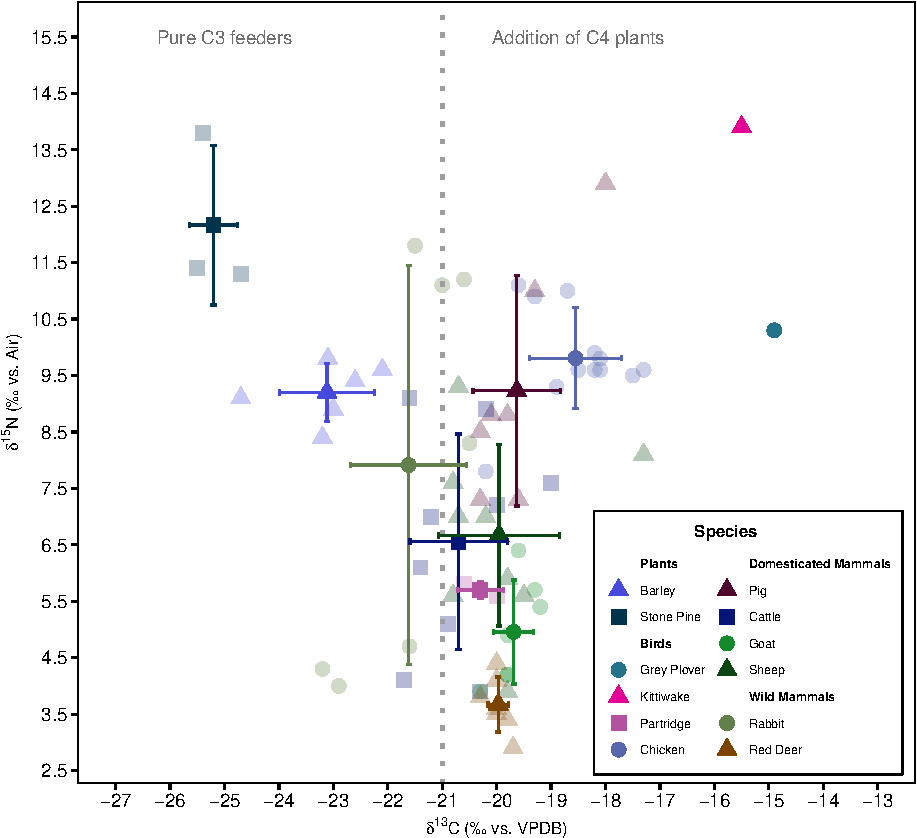
\includegraphics[width=0.98\textwidth]{castro_main_body_files/figure-latex/fauna-carbnitro-iso-plot-1} \caption{Plot showing mean \(\delta ^{13}C\) and \(\delta ^{15}N\) values (mean ± 1 SD range) of faunal bone collagen. The colour palette is produced with the Colorgorical web app (\protect\hyperlink{ref-gramazio_etal17}{Gramazio et al., 2017}).}\label{fig:fauna-carbnitro-iso-plot}
\end{figure*}

\hypertarget{wild-fauna-mammals}{%
\subsubsection{Wild fauna (mammals)}\label{wild-fauna-mammals}}

All fifty faunal samples, demonstrate (Table \ref{tab:table4}) stable isotope values within the range expected for a C\textsubscript{3} temperate ecosystem. The mean \(\delta ^{13}C\) and \(\delta ^{15}N\) values of red deer are -20 ± 0.2\text{\textperthousand} and 3.7 ± 0.5\text{\textperthousand} respectively. The other undomesticated mammal is the rabbit which has mean \(\delta ^{13}C\) values of -21.6 ± 1.1\text{\textperthousand} and mean \(\delta ^{15}N\) values of 7.9 ± 3.5\text{\textperthousand}. The mean \(\delta ^{13}C\) values of red deer are significantly higher than those of rabbits (t-statistic: -4.01, degrees of freedom: 12, \emph{p}-value: 0). This can be attributed to the rabbits' foraging ground level flora with high recycling of CO\textsubscript{2} and shade from the higher levels of the canopy in contrast with the red deer foraging at greater heights. Feeding in forested areas causes the \(\delta ^{13}C\) values to deplete due to the canopy effect (\protect\hyperlink{ref-bonafini_etal13}{Bonafini et al., 2013}). The \(\delta ^{15}N\) values of rabbits are anomalous with a standard deviation spanning almost a trophic level (standard deviation of \(\delta ^{15}N\): 3.5\text{\textperthousand}). It can be observed from Fig. \ref{fig:fauna-carbnitro-iso-plot} that the rabbits consist of two distinct groups, indicative that the group with higher \(\delta ^{13}C\) and \(\delta ^{15}N\) values was foraging in coastal/salt-marsh zones, whereas the other group had more inland located food sources (Figure \ref{fig:fauna-carbnitro-iso-plot}).

\hypertarget{domesticated-fauna-mammals}{%
\subsubsection{Domesticated fauna (mammals)}\label{domesticated-fauna-mammals}}

Sheep show mean \(\delta ^{13}C\) values of -20 ± 1.1\text{\textperthousand} and mean \(\delta ^{15}N\) values of 6.7 ± 1.6\text{\textperthousand}, while goats exhibit mean \(\delta ^{13}C\) values of -19.7 ± 0.4\text{\textperthousand} and mean \(\delta ^{15}N\) values of 5 ± 0.9\text{\textperthousand}. Goat mean \(\delta ^{13}C\) values are not significantly different from those of sheep (t-statistic: 0.61, degrees of freedom: 14, \emph{p}-value: 0.55). The ovicaprids' statistically similar mean \(\delta ^{13}C\) values indicate similar foraging in open forests (due to slightly positive \(\delta ^{13}C\) values). Sheep exhibit significantly higher \(\delta ^{15}N\) values than goats (t-statistic: 2.5, degrees of freedom: 14, \emph{p}-value: 0.03), demonstrating that sheep were foddered on food sourced from manured vegetation with the assumption of uniform coastal impact on all vegetation (Figure \ref{fig:fauna-carbnitro-iso-plot}). Sheep are superior to goats both in terms of secondary products and ease of management (\protect\hyperlink{ref-davis07}{Davis, 2007}; \protect\hyperlink{ref-rutter02}{Rutter, 2002}). Owing to the more attached economic interests with sheep, it is natural to give food sourced from cultivated crops. Since the coastal/salt marsh effect masks the increase of \(\delta ^{15}N\) values caused by manuring in cultivated crops, the statistically significant difference of \(\delta ^{15}N\) between goats and sheep can be attributed to the consumption of manured crops. Cattle show mean \(\delta ^{13}C\) values of -20.7 ± 0.9\text{\textperthousand} and mean \(\delta ^{15}N\) values of 6.6 ± 1.9\text{\textperthousand}. The cattle have statistically non-significant (t-statistic: -1.57, degrees of freedom: 16, \emph{p}-value: 0.14) \(\delta ^{13}C\) isotope ratios compared to sheep. Cattle also seem to have grazed in open areas similar to the sheep. The \(\delta ^{15}N\) isotope ratios of cattle are also significantly not different from sheep (t-statistic: 0.13, degrees of freedom: 16, \emph{p}-value: 0.9). Though significantly not different than sheep, the mean \(\delta ^{15}N\) values of cattle are lower (Figure \ref{fig:fauna-carbnitro-iso-plot}). Most of the cattle bones are from adults, which indicates that they were used as a source of power and only slaughtered for meat towards the end of their lives (\protect\hyperlink{ref-davis07}{Davis, 2007}). Since they were used for labour intense tasks, their diet could have a considerable amount of cultivated crop components. Pigs show mean \(\delta ^{13}C\) values of -19.6 ± 0.8\text{\textperthousand} and mean \(\delta ^{15}N\) values of 9.2 ± 2\text{\textperthousand}. The high \(\delta ^{15}N\) values of pigs reflect an omnivorous diet consisting of agricultural components and human food scraps similar to the Neolithic and Chalcolithic periods from Portugal (\protect\hyperlink{ref-waterman_etal16}{Waterman et al., 2016}; \protect\hyperlink{ref-zalaite_etal18}{Žalaitė et al., 2018}).

\hypertarget{wild-and-domesticated-birds}{%
\subsubsection{Wild and domesticated birds}\label{wild-and-domesticated-birds}}

Partridges show mean \(\delta ^{13}C\) values of -20.3 ± 0.4\text{\textperthousand} and mean \(\delta ^{15}N\) values of 5.7 ± 0.1\text{\textperthousand} while chicken exhibit mean \(\delta ^{13}C\) values of -18.6 ± 0.8\text{\textperthousand} and mean \(\delta ^{15}N\) values of 9.8 ± 0.9\text{\textperthousand}. The \(\delta ^{13}C\) values (t-statistic: 2.8, degrees of freedom: 12, \emph{p}-value: 0.02) and \(\delta ^{15}N\) values (t-statistic: 6.26, degrees of freedom: 12, \emph{p}-value: \ensuremath{4\times 10^{-5}}) are significantly different. The chicken owing to its domesticated status, has higher \(\delta ^{13}C\) and \(\delta ^{15}N\) values. In Iron Age, chickens were usually reared in domestic spaces while being fed on food scraps and possibly millet (a C\textsubscript{4} plant) (\protect\hyperlink{ref-fernandez-crespo_etal19}{Fernández-Crespo et al., 2019}). Chicken also eat insects alongside the human-provided food which can lead to an increase of \(\delta ^{15}N\) values. Usual partridge diet consists of arthropods, grass seeds, flowers, and weeds while they prefer foraging at the edges of agricultural fields (\protect\hyperlink{ref-green84}{Green, 1984}) which can explain the higher \(\delta ^{15}N\) values in comparison with red deer. All the partridges recovered are adults, whereas the chickens constitute juvenile-adult mix, further indicative that the former were hunted for consumption. Grey plover has a mean \(\delta ^{13}C\) value of -14.9\text{\textperthousand} and a mean \(\delta ^{15}N\) value of 10.3\text{\textperthousand}. Grey plovers are known to feed in muddy intertidal zones on insects (such as Coleoptera), polychaetes, molluscs, and crustaceans (\protect\hyperlink{ref-perez-hurtado_etal97}{Perez-Hurtado et al., 1997}). The isotope values are consistent with a diet including both terrestrial and marine prey. Kittiwake has a mean \(\delta ^{13}C\) value of -15.5\text{\textperthousand} and a mean \(\delta ^{15}N\) value of 13.9\text{\textperthousand}. Kittiwake's diet consists of fish, marine invertebrates, and plankton (\protect\hyperlink{ref-bull_etal04}{Bull et al., 2004}). The \(\delta ^{13}C\) and \(\delta ^{15}N\) values are as expected of a species with a marine diet.

Overall, the domesticated mammals are not above one trophic level (\textless{} 4\text{\textperthousand} \(\delta^{15}N\)) over the plants (both cultivated barley and stone pine) (Figure \ref{fig:fauna-carbnitro-iso-plot}). Thus, they seem to be foraging in areas away from the coastal/salt-marsh zones. Inland Iron Age domesticated mammals have mean \(\delta ^{13}C\) values ranging between 21 - 23\text{\textperthousand} (for C\textsubscript{3} temperate ecosystem) and \(\delta ^{15}N\) mean values ranging between 3-5\text{\textperthousand} for herbivores and \textgreater{} 6\text{\textperthousand} for omnivores (\protect\hyperlink{ref-fernandez-crespo_etal19}{Fernández-Crespo et al., 2019}; \protect\hyperlink{ref-hamilton_etal19}{Hamilton et al., 2019}; \protect\hyperlink{ref-schulting_etal19}{Schulting et al., 2019}; \protect\hyperlink{ref-styring_etal17}{Styring et al., 2017}). In comparison, the fauna at Castro Marim have similar \(\delta ^{13}C\) values and slightly higher \(\delta ^{15}N\) mean values. Apart from manuring, another reason for these slightly higher \(\delta^{15}N\) values could be periodic movement to a territory away from the coast. Since Iron Age Castro Marim settlement was short of foraging space (Figure \ref{fig:castro-marim-pal}), the animals could be in a periodic movement between the settlement and a space more inland. This movement can be investigated further by sequential sampling of faunal enamel for future \(\delta^{13}C_{carbonate}\) and \(\delta^{18}O\) studies (\protect\hyperlink{ref-vaiglova_etal20}{Vaiglova et al., 2020}). Any substantial increase in \(\delta^{15}N\) gained due to salt marsh foraging (\protect\hyperlink{ref-britton_etal08}{Britton et al., 2008}) or physiological stress from saline water (\protect\hyperlink{ref-ambrose91}{Ambrose, 1991}) would be evened by the subsequent migration towards inland of the domesticated fauna leading to slightly higher \(\delta ^{15}N\) values.



\begin{figure*}
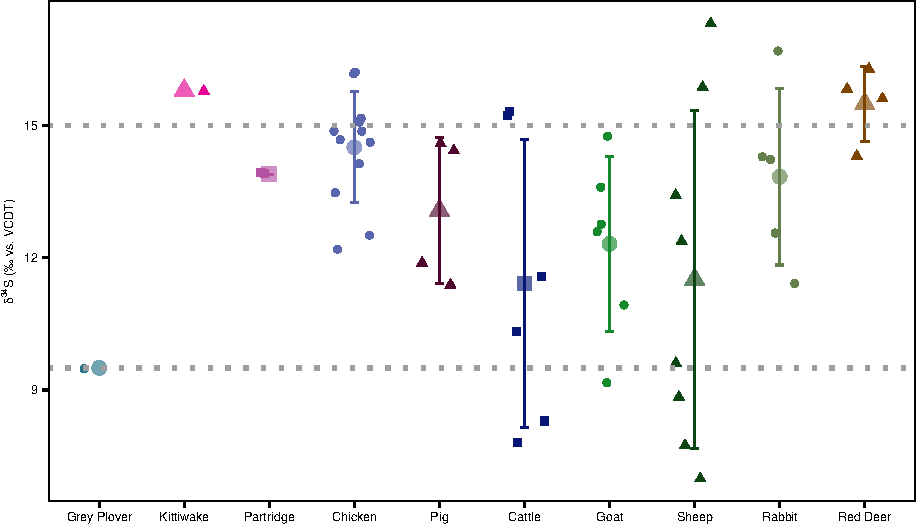
\includegraphics[width=0.98\textwidth]{castro_main_body_files/figure-latex/fauna-sulph-iso-plot-1} \caption{Plot showing mean \(\delta ^{34}S\) values (mean ± 1 SD range) of faunal bone collagen. The values are horizontally jittered to increase the visibility of the data points. The region between the gray lines represents Western European Triassic sediment \(\delta ^{34}S\) value range.}\label{fig:fauna-sulph-iso-plot}
\end{figure*}

\hypertarget{sulphur}{%
\subsection{\texorpdfstring{Faunal bone collagen \(\delta ^{34}S\) values}{Faunal bone collagen \textbackslash delta \^{}\{34\}S values}}\label{sulphur}}

\(\delta ^{34}S\) values of fauna range from 9.5 \text{\textperthousand} to 15.8 \text{\textperthousand}. The offset of \(\delta ^{34}S\) between diet to collagen is considered to be negligible (\protect\hyperlink{ref-nehlich15}{Nehlich, 2015}). Since the diet-collagen offset is negligible, collagen \(\delta ^{34}S\) values often reflect the local geological settings and sea-spray due to proximity to the coast (\textless30 km). The geological substrate of areas surrounding Castro Marim consists of patches of Triassic sediments surrounded by Quaternary bedrock zones (\protect\hyperlink{ref-terrinha98}{Terrinha, 1998}). A compilation of \(\delta ^{34}S\) of Triassic sediments from Western Europe (\protect\hyperlink{ref-claypool_etal80}{Claypool et al., 1980}) presents a range of 9.5\text{\textperthousand} to 15\text{\textperthousand}. Thus, any values between this range can be considered as a signal for local. Both grey plover and kittiwake are known to migrate seasonally, which makes the interpretation of their \(\delta ^{34}S\) values complicated (\protect\hyperlink{ref-coulson11}{Coulson, 2011}; \protect\hyperlink{ref-thompsonbyrkjedal10}{Thompson and Byrkjedal, 2010}). Kittiwake has higher \(\delta ^{34}S\) value than the Triassic range that can attributed to its highly marine diet, indicated by its \(\delta ^{13}C\) and \(\delta ^{15}N\) values. The average \(\delta ^{34}S\) values of all other fauna fall within the range of Western European Triassic sediments, thus indicating that most of them are of local origin (Figure \ref{fig:fauna-sulph-iso-plot}). Though some animals (two chicken, four cattle, five sheep, one goat, one rabbit, and two red deer) yield \(\delta ^{34}S\) values outside the Triassic range. This could be due to these individuals originating from a different geological bedrock. \(\delta ^{34}S\) mean values of rabbits are 13.8 ± 2\text{\textperthousand}, and the \(\delta ^{34}S\) mean values of red deer are 15.5 ± 0.9\text{\textperthousand}. Both the wild mammals have low standard deviations indicating that individuals are of close spatial origins or with similar bedrocks (Figure \ref{fig:fauna-sulph-iso-plot}). From the domesticated species, goats have mean \(\delta ^{34}S\) values of 12.3 ± 2\text{\textperthousand}, pigs have mean \(\delta ^{34}S\) values of 13.1 ± 1.7\text{\textperthousand}, and chickens have mean \(\delta ^{34}S\) values of 14.5 ± 1.3\text{\textperthousand}. These three species have relatively low standard deviations similar to wild mammals (Figure \ref{fig:fauna-sulph-iso-plot}). Pigs and chicken could have been penned in spaces attached to human residences, giving rise to the low standard deviations. The \(\delta ^{34}S\) values of goats can be explained by foraging in areas with similar bedrocks. In the case of sheep, the mean \(\delta ^{34}S\) values are 11.5 ± 3.8\text{\textperthousand} while the mean \(\delta ^{34}S\) values of cattle are 11.4 ± 3.3\text{\textperthousand}. Sheep and cattle have the highest standard deviation amongst the fauna, which could be caused due to periodic movement between areas with different bedrocks (Figure \ref{fig:castro-marim-loc} and Figure \ref{fig:fauna-sulph-iso-plot}). Since the average \(\delta ^{34}S\) values of sheep and cattle are still within the range of what is considered local, the movement could be somewhere inland within the territory of the settlement.

\hypertarget{conclusions}{%
\section{Conclusions}\label{conclusions}}

The \(\delta ^{13}C\) values of the two barley cultivars indicate complete dependence on natural precipitation with little to no artificial irrigation. In the case of stone pine, \(\delta ^{13}C\) values are non-conclusive concerning watering status due to the lack of established studies for \emph{Pinus} species. The \(\delta ^{15}N\) ratios of the plants are elevated due to the proximity of coast/salt marsh. The manuring of barley was masked by the high nitrogen nutrient soils of the salt marshes but manuring of crops fed to ovicaprids can be inferred from the significant difference between the mean \(\delta ^{15}N\) values of sheep and goats. The \(\delta ^{15}N\) values of stone pine are greater than those of the barley, indicating that the cultivation took place in locations far away from coast/salt marsh which is evident from the absence of space near the settlement in Iron Age. In the case of wild fauna, the \(\delta ^{13}C\) values of rabbits indicate foraging at ground level in closed settings, while those of red deer indicate grazing at higher levels in more open areas. The \(\delta ^{15}N\) values of rabbits indicate two different groups, with one group foraging in salt marshes and the other from a more terrestrial setting. Ovicaprid \(\delta ^{13}C\) values indicate foraging in open pastures. Comparing the \(\delta ^{15}N\) ratios of sheep and goats show that the former was fed agricultural produce/by-products, which the latter lacked. The cattle also foraged in open areas and had cultivated components in its diet compared to the sheep. Pigs exhibit \(\delta ^{13}C\) and \(\delta ^{15}N\) values consistent with an omnivorous diet. In the case of the seabirds, both grey plover and kittiwake exhibit \(\delta ^{13}C\) and \(\delta ^{15}N\) values consistent with their diet. Chicken has \(\delta ^{13}C\) and \(\delta ^{15}N\) values are reflective of its domesticated status with a mixture of C\textsubscript{3} and C\textsubscript{4} plants, insects, and food scraps. The \(\delta ^{15}N\) values of the fauna are not a trophic level above the plants, which can be because of either periodic movement or salt stress. The \(\delta ^{34}S\) values of overall fauna indicate a local origin. Goats, pigs, and chickens have a low range of values due to penning in domestic spaces. The \(\delta ^{34}S\) values of cattle and sheep have a more extensive range of values which could be due to periodic migration or of being non-local origin.

This study is the first of its kind on Phoenician-Punic fauna from the Iberian Peninsula. The study has given a preliminary insight into the cultivation and husbandry practices in Castro Marim during the Iron Age. The stable isotope data has also raised the possibility of transhumance at Castro Marim, which can only be answered in future studies.

\hypertarget{acknowledgements}{%
\section{Acknowledgements}\label{acknowledgements}}

This project has received funding from the European Union's Horizon 2020 research and innovation programme under the Marie Skłodowska-Curie grant agreement No.~766311. The ZooMS analysis was carried out by Samantha Presslee at BioArCh, University of York who gratefully acknowledges the use of the Ultraflex III MALDI-ToF/ToF instrument in the York Centre of Excellence in Mass Spectrometry. The centre was created thanks to a major capital investment through Science City York, supported by Yorkshire Forward with funds from the Northern Way Initiative, and subsequent support from EPSRC (EP/K039660/1; EP/M028127/1). The authors would like to thank Rui Parreira for providing access to the samples (Direção Regional de Cultura do Algarve, Faro).

\hypertarget{references}{%
\section*{References}\label{references}}
\addcontentsline{toc}{section}{References}

\hypertarget{refs}{}
\begin{CSLReferences}{1}{0}
\leavevmode\vadjust pre{\hypertarget{ref-ambrose91}{}}%
Ambrose, S.H., 1991. Effects of diet, climate and physiology on nitrogen isotope abundances in terrestrial foodwebs. Journal of Archaeological Science 18, 293--317. \url{https://doi.org/10.1016/0305-4403(91)90067-Y}

\leavevmode\vadjust pre{\hypertarget{ref-ambrose90}{}}%
Ambrose, S.H., 1990. Preparation and characterization of bone and tooth collagen for isotopic analysis. Journal of Archaeological Science 17, 431--451. \url{https://doi.org/10.1016/0305-4403(90)90007-R}

\leavevmode\vadjust pre{\hypertarget{ref-arrastio00}{}}%
Arrastio, F.J.M., 2000. Tartessos, estelas, modelos pesimistas, in: Intercambio y Comercio Preclásico En El {Mediterráneo}: Actas Del {I} Coloquio Del {CEFYP}, {Madrid}, 9-12 de Noviembre, 1998. {Centro de Estudios Fenicios y Púnicos}, pp. 153--174.

\leavevmode\vadjust pre{\hypertarget{ref-arrastio99}{}}%
Arrastio, F.J.M., 1999. Conflictos y perspectivas en el periodo precolonial tartésico. Gerión. Revista de Historia Antigua 17, 149.

\leavevmode\vadjust pre{\hypertarget{ref-arruda09}{}}%
Arruda, A.M., 2009. Phoenician colonization on the {Atlantic Coast} of the {Iberian Peninsula}. {Chicago: The University of Chicago Press, 2009.}

\leavevmode\vadjust pre{\hypertarget{ref-arruda03}{}}%
Arruda, A.M., 2003. Contributo da colonização fenícia para a domesticação da terra portuguesa. Ecohistoria del paisaje agrario-la agricultura fenicio-púnica en el mediterráneo.

\leavevmode\vadjust pre{\hypertarget{ref-arruda00}{}}%
Arruda, A.M., 2000. Los fenicios en {Portugal}. {Fenicios} y mundo indígena en el centro y sur de {Portugal} (siglos {VIII}-{VI aC}). {Universidad Pompeu Fabra de Barcelona/Carrera Edició, SL}.

\leavevmode\vadjust pre{\hypertarget{ref-arruda97}{}}%
Arruda, A.M., 1997. Os núcleos urbanos litorais da {Idade} do {Ferro} no {Algarve}. Noventa Séculos entre a Serra e o Mar 243--255.

\leavevmode\vadjust pre{\hypertarget{ref-arruda96}{}}%
Arruda, A.M., 1996. O {Castelo} de {Castro Marim}, in: In {De Ulisses} a {Viriato}. {O} Primeiro Milénio a.{C}.. {Ministério da Cultura, Instituto Português de Museus, Museu Nacional de Arqueologia}, {Lisboa}, pp. 95--100.

\leavevmode\vadjust pre{\hypertarget{ref-arruda_etal20}{}}%
Arruda, A.M., Ferreira, D., Sousa, E. de, 2020. A cerâmica grega do {Castelo} de {Castro Marim}. {UNIARQ. Centro de Arqueologia da Universidade de Lisboa}.

\leavevmode\vadjust pre{\hypertarget{ref-arruda_freitas08}{}}%
Arruda, A.M., Freitas, V.T. de, 2008. \href{https://repositorio.ul.pt/handle/10451/9778}{O castelo de castro marim durante os séculos VI e v a.n.e.} Sidereum Ana I: El río Guadiana en época Post-Orientalizante. 429--446.

\leavevmode\vadjust pre{\hypertarget{ref-arruda_etal13}{}}%
Arruda, A.M., Soares, A.M., Freitas, V.T. de, Oliveira, C.F., Martins, J.M.M., Portela, P.J., 2013. A cronologia relativa e absoluta da ocupação sidérica do {Castelo} de {Castro Marim}. Saguntum 45, 101--114.

\leavevmode\vadjust pre{\hypertarget{ref-arruda_etal06}{}}%
Arruda, A.M., Viegas, C., Bargão, P., Pereira, R., 2006. A importação de preparados de peixe em {Castro Marim}: Da {Idade} do {Ferro} á {Época Romana}. Setúbal Arqueológica 13, 153--176.

\leavevmode\vadjust pre{\hypertarget{ref-aubet01}{}}%
Aubet, M.E., 2001. The {Phoenicians} and the {West}: Politics, colonies and trade. {Cambridge Univ. Press}.

\leavevmode\vadjust pre{\hypertarget{ref-aubet87}{}}%
Aubet, M.E., 1987. Tiro y las colonias fenicias de {Occidente}. {Ed. Bellaterra}.

\leavevmode\vadjust pre{\hypertarget{ref-bocherens_drucker03}{}}%
Bocherens, H., Drucker, D., 2003. Trophic level isotopic enrichment of carbon and nitrogen in bone collagen: Case studies from recent and ancient terrestrial ecosystems. International Journal of Osteoarchaeology 13, 46--53. \url{https://doi.org/10.1002/oa.662}

\leavevmode\vadjust pre{\hypertarget{ref-boessneck_etal64}{}}%
Boessneck, J., Müller, H.-H., Teichert, M., 1964. Osteologische {Unterscheidungsmerkmale} zwischen {Schaf} ({Ovis} aries {Linné}) und {Ziege} ({Capra} hircus {Linné}). {Verlag nicht ermittelbar}.

\leavevmode\vadjust pre{\hypertarget{ref-bogaard_etal13}{}}%
Bogaard, A., Fraser, R., Heaton, T.H.E., Wallace, M., Vaiglova, P., Charles, M., Jones, G., Evershed, R.P., Styring, A.K., Andersen, N.H., Arbogast, R.-M., Bartosiewicz, L., Gardeisen, A., Kanstrup, M., Maier, U., Marinova, E., Ninov, L., Schäfer, M., Stephan, E., 2013. Crop manuring and intensive land management by {Europe}'s first farmers. PNAS 110, 12589--12594. \url{https://doi.org/10.1073/pnas.1305918110}

\leavevmode\vadjust pre{\hypertarget{ref-bogaard_etal07}{}}%
Bogaard, A., Heaton, T.H.E., Poulton, P., Merbach, I., 2007. The impact of manuring on nitrogen isotope ratios in cereals: Archaeological implications for reconstruction of diet and crop management practices. Journal of Archaeological Science 34, 335--343. \url{https://doi.org/10.1016/j.jas.2006.04.009}

\leavevmode\vadjust pre{\hypertarget{ref-bonafini_etal13}{}}%
Bonafini, M., Pellegrini, M., Ditchfield, P., Pollard, A.M., 2013. Investigation of the 'canopy effect' in the isotope ecology of temperate woodlands. Journal of Archaeological Science 40, 3926--3935. \url{https://doi.org/10.1016/j.jas.2013.03.028}

\leavevmode\vadjust pre{\hypertarget{ref-britton_etal08}{}}%
Britton, K., Mldner, G., Bell, M., 2008. Stable isotope evidence for salt-marsh grazing in the {Bronze Age Severn Estuary}, {UK}: Implications for palaeodietary analysis at coastal sites. Journal of Archaeological Science 35, 2111--2118. \url{https://doi.org/10.1016/j.jas.2008.01.012}

\leavevmode\vadjust pre{\hypertarget{ref-buckley_etal09}{}}%
Buckley, M., Collins, M., Thomas‐Oates, J., Wilson, J.C., 2009. Species identification by analysis of bone collagen using matrix-assisted laser desorption/ionisation time-of-flight mass spectrometry. Rapid Communications in Mass Spectrometry 23, 3843--3854. \url{https://doi.org/10.1002/rcm.4316}

\leavevmode\vadjust pre{\hypertarget{ref-buckley_etal10}{}}%
Buckley, M., Whitcher Kansa, S., Howard, S., Campbell, S., Thomas-Oates, J., Collins, M., 2010. Distinguishing between archaeological sheep and goat bones using a single collagen peptide. Journal of Archaeological Science 37, 13--20. \url{https://doi.org/10.1016/j.jas.2009.08.020}

\leavevmode\vadjust pre{\hypertarget{ref-bull_etal04}{}}%
Bull, J., Wanless, S., Elston, D.A., Daunt, F., Lewis, S., Harris, M.P., J, B., Wanless, S., Elston, D.A., Daunt, F., Lewis, S., Harris, M.P., 2004. Local-scale variability in the diet of {Black}-legged {Kittiwakes Rissa} tridactyla. Ardea 43--52.

\leavevmode\vadjust pre{\hypertarget{ref-claypool_etal80}{}}%
Claypool, G.E., Holser, W.T., Kaplan, I.R., Sakai, H., Zak, I., 1980. The age curves of sulfur and oxygen isotopes in marine sulfate and their mutual interpretation. Chemical Geology 28, 199--260. \url{https://doi.org/10.1016/0009-2541(80)90047-9}

\leavevmode\vadjust pre{\hypertarget{ref-cloern_etal02}{}}%
Cloern, J.E., Canuel, E.A., Harris, D., 2002. Stable carbon and nitrogen isotope composition of aquatic and terrestrial plants of the {San Francisco Bay} estuarine system. Limnology and Oceanography 47, 713--729. \url{https://doi.org/10.4319/lo.2002.47.3.0713}

\leavevmode\vadjust pre{\hypertarget{ref-coulson11}{}}%
Coulson, J., 2011. The kittiwake. {A\&C Black}.

\leavevmode\vadjust pre{\hypertarget{ref-davis07}{}}%
Davis, S., 2007. The mammals and birds from the {Iron Age} and {Roman} periods of {Castro Marim}, {Algarve}, {Portugal}. Trabalhos do CIPA 107.

\leavevmode\vadjust pre{\hypertarget{ref-deniro_epstein81}{}}%
Deniro, M.J., Epstein, S., 1981. Influence of diet on the distribution of nitrogen isotopes in animals. Geochimica et Cosmochimica Acta 45, 341--351. \url{https://doi.org/10.1016/0016-7037(81)90244-1}

\leavevmode\vadjust pre{\hypertarget{ref-deniro85}{}}%
DeNiro, M.J., 1985. Postmortem preservation and alteration of in vivo bone collagen isotope ratios in relation to palaeodietary reconstruction. Nature 317, 806--809. \url{https://doi.org/10.1038/317806a0}

\leavevmode\vadjust pre{\hypertarget{ref-deniro_epstein78}{}}%
DeNiro, M.J., Epstein, S., 1978. Influence of diet on the distribution of carbon isotopes in animals. Geochimica et Cosmochimica Acta 42, 495--506. \url{https://doi.org/10.1016/0016-7037(78)90199-0}

\leavevmode\vadjust pre{\hypertarget{ref-dietler09}{}}%
Dietler, M., 2009. Colonial encounters in {Iberia} and the {Western Mediterranean}: {An} exploratory framework.

\leavevmode\vadjust pre{\hypertarget{ref-dixon06}{}}%
Dixon, G.R., 2006. Origins and diversity of {Brassica} and its relatives., in: Dixon, G.R. (Ed.), Vegetable Brassicas and Related Crucifers. {CABI}, {Wallingford}, pp. 1--33. \url{https://doi.org/10.1079/9780851993959.0001}

\leavevmode\vadjust pre{\hypertarget{ref-eshel_etal19}{}}%
Eshel, T., Erel, Y., Yahalom-Mack, N., Tirosh, O., Gilboa, A., 2019. Lead isotopes in silver reveal earliest {Phoenician} quest for metals in the west {Mediterranean}. Proc Natl Acad Sci USA 116, 6007. \url{https://doi.org/10.1073/pnas.1817951116}

\leavevmode\vadjust pre{\hypertarget{ref-farquhar_etal89}{}}%
Farquhar, G.D., Ehleringer, J.R., Hubick, K.T., 1989. Carbon {Isotope Discrimination} and {Photosynthesis}. Annu. Rev. Plant. Physiol. Plant. Mol. Biol. 40, 503--537. \url{https://doi.org/10.1146/annurev.pp.40.060189.002443}

\leavevmode\vadjust pre{\hypertarget{ref-farquhar_etal82}{}}%
Farquhar, G., O'Leary, M., Berry, J., 1982. On the {Relationship Between Carbon Isotope Discrimination} and the {Intercellular Carbon Dioxide Concentration} in {Leaves}. Functional Plant Biol. 9, 121. \url{https://doi.org/10.1071/PP9820121}

\leavevmode\vadjust pre{\hypertarget{ref-fernandez-crespo_etal19}{}}%
Fernández-Crespo, T., Ordoño, J., Bogaard, A., Llanos, A., Schulting, R., 2019. A snapshot of subsistence in {Iron Age Iberia}: {The} case of {La Hoya} village. Journal of Archaeological Science: Reports 28, 102037. \url{https://doi.org/10.1016/j.jasrep.2019.102037}

\leavevmode\vadjust pre{\hypertarget{ref-ferrio_etal05}{}}%
Ferrio, J.P., Araus, J.L., Buxó, R., Voltas, J., Bort, J., 2005. Water management practices and climate in ancient agriculture: Inferences from the stable isotope composition of archaeobotanical remains. Veget Hist Archaeobot 14, 510--517. \url{https://doi.org/10.1007/s00334-005-0062-2}

\leavevmode\vadjust pre{\hypertarget{ref-ferrio_etal07}{}}%
Ferrio, J.P., Voltas, J., Alonso, N., Araus, J.L., 2007. Reconstruction of {Climate} and {Crop Conditions} in the {Past Based} on the {Carbon Isotope Signature} of {Archaeobotanical Remains}, in: Terrestrial {Ecology}. {Elsevier}, pp. 319--332. \url{https://doi.org/10.1016/S1936-7961(07)01020-2}

\leavevmode\vadjust pre{\hypertarget{ref-fiorentino_etal15}{}}%
Fiorentino, G., Ferrio, J.P., Bogaard, A., Araus, J.L., Riehl, S., 2015. Stable isotopes in archaeobotanical research. Veget Hist Archaeobot 24, 215--227. \url{https://doi.org/10.1007/s00334-014-0492-9}

\leavevmode\vadjust pre{\hypertarget{ref-fletcher_etal07}{}}%
Fletcher, W.J., Boski, T., Moura, D., 2007. Palynological evidence for environmental and climatic change in the lower {Guadiana} valley, {Portugal}, during the last 13 000 years. The Holocene 17, 481--494. \url{https://doi.org/10.1177/0959683607077027}

\leavevmode\vadjust pre{\hypertarget{ref-fraser_etal13a}{}}%
Fraser, R.A., Bogaard, A., Charles, M., Styring, A.K., Wallace, M., Jones, G., Ditchfield, P., Heaton, T.H.E., 2013. Assessing natural variation and the effects of charring, burial and pre-treatment on the stable carbon and nitrogen isotope values of archaeobotanical cereals and pulses. Journal of Archaeological Science 40, 4754--4766. \url{https://doi.org/10.1016/j.jas.2013.01.032}

\leavevmode\vadjust pre{\hypertarget{ref-fraser_etal11}{}}%
Fraser, R.A., Bogaard, A., Heaton, T., Charles, M., Jones, G., Christensen, B.T., Halstead, P., Merbach, I., Poulton, P.R., Sparkes, D., Styring, A.K., 2011. Manuring and stable nitrogen isotope ratios in cereals and pulses: Towards a new archaeobotanical approach to the inference of land use and dietary practices. Journal of Archaeological Science 38, 2790--2804. \url{https://doi.org/10.1016/j.jas.2011.06.024}

\leavevmode\vadjust pre{\hypertarget{ref-froehle_etal10}{}}%
Froehle, A.W., Kellner, C.M., Schoeninger, M.J., 2010. {FOCUS}: Effect of diet and protein source on carbon stable isotope ratios in collagen: Follow up to {Warinner} and {Tuross} (2009). Journal of Archaeological Science 37, 2662--2670. \url{https://doi.org/10.1016/j.jas.2010.06.003}

\leavevmode\vadjust pre{\hypertarget{ref-gale_carruthers00}{}}%
Gale, R., Carruthers, W., 2000. Charcoal and charred seed remains from {Middle Palaeolithic} levels at {Gorham}'s and {Vanguard Caves}. Neanderthals on the Edge. Oxford: Oxbow Books 207--210.

\leavevmode\vadjust pre{\hypertarget{ref-gomes_arruda18}{}}%
Gomes, F.B., Arruda, A.M., 2018. On the edge of history? {The Early Iron Age} of southern {Portugal}, between texts and archaeology. World Archaeology 50, 764--780. \url{https://doi.org/10.1080/00438243.2019.1604258}

\leavevmode\vadjust pre{\hypertarget{ref-gomezbellard19}{}}%
Gómez Bellard, C., 2019. Agriculture, in: The {Oxford Handbook} of {The Phoenician} and {Punic Mediterranean}. {Oxford University Press}, pp. 732--745.

\leavevmode\vadjust pre{\hypertarget{ref-gramazio_etal17}{}}%
Gramazio, C.C., Laidlaw, D.H., Schloss, K.B., 2017. Colorgorical: {Creating} discriminable and preferable color palettes for information visualization. IEEE Trans. Visual. Comput. Graphics 23, 521--530. \url{https://doi.org/10.1109/TVCG.2016.2598918}

\leavevmode\vadjust pre{\hypertarget{ref-green84}{}}%
Green, R.E., 1984. The {Feeding Ecology} and {Survival} of {Partridge Chicks} ({Alectoris} rufa and {Perdix} perdix) on {Arable Farmland} in {East Anglia}. Journal of Applied Ecology 21, 817--830. \url{https://doi.org/10.2307/2405049}

\leavevmode\vadjust pre{\hypertarget{ref-hamilton_etal19}{}}%
Hamilton, W.D., Sayle, K.L., Boyd, M.O.E., Haselgrove, C.C., Cook, G.T., 2019. {``{Celtic} cowboys''} reborn: Application of multi-isotopic analysis ({\(\delta^{13}\)C}, {\(\delta^{15}\)N}, and {\(\delta^{34}\)S}) to examine mobility and movement of animals within an {Iron Age British} society. Journal of Archaeological Science 101, 189--198. \url{https://doi.org/10.1016/j.jas.2018.04.006}

\leavevmode\vadjust pre{\hypertarget{ref-haws04}{}}%
Haws, J., 2004. An {Iberian} perspective on {Upper Paleolithic} plant consumption. Promontoria 2, 49--106.

\leavevmode\vadjust pre{\hypertarget{ref-heaton87}{}}%
Heaton, T.H.E., 1987. The \(^{15}N\)/\(^{14}N\) ratios of plants in {South Africa} and {Namibia}: Relationship to climate and coastal/saline environments. Oecologia 74, 236--246. \url{https://doi.org/10.1007/BF00379365}

\leavevmode\vadjust pre{\hypertarget{ref-hedges_reynard07}{}}%
Hedges, R.E.M., Reynard, L.M., 2007. Nitrogen isotopes and the trophic level of humans in archaeology. Journal of Archaeological Science 34, 1240--1251. \url{https://doi.org/10.1016/j.jas.2006.10.015}

\leavevmode\vadjust pre{\hypertarget{ref-hobson99}{}}%
Hobson, K.A., 1999. Tracing origins and migration of wildlife using stable isotopes: A review. Oecologia 120, 314--326. \url{https://doi.org/10.1007/s004420050865}

\leavevmode\vadjust pre{\hypertarget{ref-hollund_etal13}{}}%
Hollund, H.I., Ariese, F., Fernandes, R., Jans, M.M.E., Kars, H., 2013. Testing an {Alternative High}-{Throughput Tool} for {Investigating Bone Diagenesis}: {Ftir} in {Attenuated Total Reflection} (atr) {Mode}*. Archaeometry 55, 507--532. \url{https://doi.org/10.1111/j.1475-4754.2012.00695.x}

\leavevmode\vadjust pre{\hypertarget{ref-jalut_etal00}{}}%
Jalut, G., Amat, A.E., Bonnet, L., Gauquelin, T., Fontugne, M., 2000. Holocene climatic changes in the {Western Mediterranean}, from south-east {France} to south-east {Spain}. Palaeogeography, Palaeoclimatology, Palaeoecology 160, 255--290.

\leavevmode\vadjust pre{\hypertarget{ref-kellner_schoeninger07}{}}%
Kellner, C.M., Schoeninger, M.J., 2007. A simple carbon isotope model for reconstructing prehistoric human diet. American Journal of Physical Anthropology 133, 1112--1127. \url{https://doi.org/10.1002/ajpa.20618}

\leavevmode\vadjust pre{\hypertarget{ref-vanklinken99}{}}%
Klinken, G.J. van, 1999. Bone {Collagen Quality Indicators} for {Palaeodietary} and {Radiocarbon Measurements}. Journal of Archaeological Science 26, 687--695. \url{https://doi.org/10.1006/jasc.1998.0385}

\leavevmode\vadjust pre{\hypertarget{ref-kohn10}{}}%
Kohn, M.J., 2010. Carbon isotope compositions of terrestrial {C3} plants as indicators of (paleo)ecology and (paleo)climate. Proc Natl Acad Sci U S A 107, 19691--19695. \url{https://doi.org/10.1073/pnas.1004933107}

\leavevmode\vadjust pre{\hypertarget{ref-lebon_etal16}{}}%
Lebon, M., Reiche, I., Gallet, X., Bellot-Gurlet, L., Zazzo, A., 2016. Rapid {Quantification} of {Bone Collagen Content} by {ATR}-{FTIR Spectroscopy}. Radiocarbon 58, 131--145. \url{https://doi.org/10.1017/RDC.2015.11}

\leavevmode\vadjust pre{\hypertarget{ref-leegood13}{}}%
Leegood, R.C., 2013. Photosynthesis, in: Lennarz, W.J., Lane, M.D. (Eds.), Encyclopedia of {Biological Chemistry} ({Second Edition}). {Academic Press}, {Waltham}, pp. 492--496. \url{https://doi.org/10.1016/B978-0-12-378630-2.00049-9}

\leavevmode\vadjust pre{\hypertarget{ref-longin71}{}}%
Longin, R., 1971. New {Method} of {Collagen Extraction} for {Radiocarbon Dating}. Nature 230, 241--242. \url{https://doi.org/10.1038/230241a0}

\leavevmode\vadjust pre{\hypertarget{ref-magny_etal02}{}}%
Magny, M., Miramont, C., Sivan, O., 2002. Assessment of the impact of climate and anthropogenic factors on {Holocene Mediterranean} vegetation in {Europe} on the basis of palaeohydrological records. Palaeogeography, Palaeoclimatology, Palaeoecology 186, 47--59.

\leavevmode\vadjust pre{\hypertarget{ref-manfredi92}{}}%
Manfredi, L.I., 1992. Le saline et il sale nel mundo punico. Rivista di Studi Fenici 20, 3--14.

\leavevmode\vadjust pre{\hypertarget{ref-markoe05}{}}%
Markoe, G.E., 2005. Phoenicians. {London}: {The British Museum}.

\leavevmode\vadjust pre{\hypertarget{ref-martin71}{}}%
Martin, R., 1971. Recherches sur les agronomes latins et leurs conceptions économiques et sociales.

\leavevmode\vadjust pre{\hypertarget{ref-nehlich15}{}}%
Nehlich, O., 2015. The application of sulphur isotope analyses in archaeological research: {A} review. Earth-Science Reviews 142, 1--17. \url{https://doi.org/10.1016/j.earscirev.2014.12.002}

\leavevmode\vadjust pre{\hypertarget{ref-nehlich_etal10}{}}%
Nehlich, O., Borić, D., Stefanović, S., Richards, M.P., 2010. Sulphur isotope evidence for freshwater fish consumption: A case study from the {Danube Gorges}, {SE Europe}. Journal of Archaeological Science 37, 1131--1139.

\leavevmode\vadjust pre{\hypertarget{ref-nehlich_richards09}{}}%
Nehlich, O., Richards, M.P., 2009. Establishing collagen quality criteria for sulphur isotope analysis of archaeological bone collagen. Archaeological and Anthropological Sciences 1, 59--75. \url{https://doi.org/10.1007/s12520-009-0003-6}

\leavevmode\vadjust pre{\hypertarget{ref-neville98}{}}%
Neville, A., 1998. The {Phoenicians} in {Iberia}: {Settlements}, {Cemetries}, {Trade} and {Agriculture}.

\leavevmode\vadjust pre{\hypertarget{ref-nitsch_etal15}{}}%
Nitsch, E.K., Charles, M., Bogaard, A., 2015. Calculating a statistically robust \(\delta ^{13}C\) and \(\delta ^{15}N\) offset for charred cereal and pulse seeds. STAR: Science \& Technology of Archaeological Research 1, 1--8. \url{https://doi.org/10.1179/2054892315Y.0000000001}

\leavevmode\vadjust pre{\hypertarget{ref-nitsch_etal19}{}}%
Nitsch, E.K., Lamb, A.L., Heaton, T.H.E., Vaiglova, P., Fraser, R., Hartman, G., Moreno-Jiménez, E., López-Piñeiro, A., Peña-Abades, D., Fairbairn, A., Eriksen, J., Bogaard, A., 2019. The {Preservation} and {Interpretation} of {\(\delta^{34}\)S Values} in {Charred Archaeobotanical Remains}. Archaeometry 61, 161--178. \url{https://doi.org/10.1111/arcm.12388}

\leavevmode\vadjust pre{\hypertarget{ref-payne69}{}}%
Payne, S., 1969. A metrical distinction between sheep and goat metacarpals. The domestication and exploitation of plants and animals 295--305.

\leavevmode\vadjust pre{\hypertarget{ref-pena-chocarro_etal19}{}}%
Peña-Chocarro, L., Pérez- Jordá, G., Alonso, N., Antolín, F., Teira-Brión, A., Tereso, J.P., Montes Moya, E.M., López Reyes, D., 2019. Roman and medieval crops in the {Iberian Peninsula}: {A} first overview of seeds and fruits from archaeological sites. Quaternary International, Food {Production} and {Land Use} 499, 49--66. \url{https://doi.org/10.1016/j.quaint.2017.09.037}

\leavevmode\vadjust pre{\hypertarget{ref-perez-hurtado_etal97}{}}%
Perez-Hurtado, A., Goss-Custard, J.D., Garcia, F., 1997. The diet of wintering waders in cádiz bay, southwest spain. Bird Study 44, 45--52. \url{https://doi.org/10.1080/00063659709461037}

\leavevmode\vadjust pre{\hypertarget{ref-price_etal17}{}}%
Price, G.C., Krigbaum, J., Shelton, K., 2017. Stable isotopes and discriminating tastes: {Faunal} management practices at the {Late Bronze Age} settlement of {Mycenae}, {Greece}. Journal of Archaeological Science: Reports 14, 116--126. \url{https://doi.org/10.1016/j.jasrep.2017.05.034}

\leavevmode\vadjust pre{\hypertarget{ref-queiroz_etal06}{}}%
Queiroz, P., Mateus, J., Leeuwaarden, W., Pereira, T., Dise, D., 2006. Castro {Marim} e o seu território imediato durante a {Antiguidade}. {Paleo}-etno-{Botânica}. {Relatório Final}. \url{https://doi.org/10.13140/RG.2.2.25361.63848}

\leavevmode\vadjust pre{\hypertarget{ref-quinn19}{}}%
Quinn, J., 2019. In search of the {Phoenicians}. {Princeton University Press}.

\leavevmode\vadjust pre{\hypertarget{ref-rcoreteam20}{}}%
R Core Team, 2020. \href{https://www.R-project.org/}{R: {A Language} and {Environment} for {Statistical Computing}}. {R Foundation for Statistical Computing}, {Vienna, Austria}.

\leavevmode\vadjust pre{\hypertarget{ref-renzi_etal12}{}}%
Renzi, M., Rovira Llorens, S., Montero Ruiz, I., 2012. Riflessioni sulla metallurgia fenicia dell'argento nella {Penisola Iberica}.

\leavevmode\vadjust pre{\hypertarget{ref-richards_hedges99}{}}%
Richards, M.P., Hedges, R.E.M., 1999. Stable {Isotope Evidence} for {Similarities} in the {Types} of {Marine Foods Used} by {Late Mesolithic Humans} at {Sites Along} the {Atlantic Coast} of {Europe}. Journal of Archaeological Science 26, 717--722. \url{https://doi.org/10.1006/jasc.1998.0387}

\leavevmode\vadjust pre{\hypertarget{ref-riehl09}{}}%
Riehl, S., 2009. Archaeobotanical evidence for the interrelationship of agricultural decision-making and climate change in the ancient {Near East}. Quaternary International 197, 93--114. \url{https://doi.org/10.1016/j.quaint.2007.08.005}

\leavevmode\vadjust pre{\hypertarget{ref-roller14}{}}%
Roller, D.W., 2014. The geography of {Strabo}: {An English} translation, with introduction and notes. {Cambridge University Press}.

\leavevmode\vadjust pre{\hypertarget{ref-rutter02}{}}%
Rutter, S.M., 2002. Behaviour of {Sheep} and {Goats}, in: The Ethology of Domestic Animals: {An} Introductory Text. pp. 148--155.

\leavevmode\vadjust pre{\hypertarget{ref-schoeninger85}{}}%
Schoeninger, M.J., 1985. Trophic level effects on {15N}/{14N} and {13C}/{12C} ratios in bone collagen and strontium levels in bone mineral. Journal of Human Evolution 14, 515--525. \url{https://doi.org/10.1016/S0047-2484(85)80030-0}

\leavevmode\vadjust pre{\hypertarget{ref-schramm67}{}}%
Schramm, Z., 1967. Morphological differences of some goat and sheep bones. {Wyższa Szkoła Rolnicza}.

\leavevmode\vadjust pre{\hypertarget{ref-schulting_etal19}{}}%
Schulting, R.J., le Roux, P., Gan, Y.M., Pouncett, J., Hamilton, J., Snoeck, C., Ditchfield, P., Henderson, R., Lange, P., Lee-Thorp, J., Gosden, C., Lock, G., 2019. The ups \& downs of {Iron Age} animal management on the {Oxfordshire Ridgeway}, south-central {England}: A multi-isotope approach. Journal of Archaeological Science 101, 199--212. \url{https://doi.org/10.1016/j.jas.2018.09.006}

\leavevmode\vadjust pre{\hypertarget{ref-semmler92}{}}%
Semmler, M.E.A., 1992. Proyecto {Cerro} del {Villar} ({Guadalhorce}, {Málaga}): Estudio de materiales 1990, in: Anuario Arqueológico de {Andalucía} 1990. pp. 304--306.

\leavevmode\vadjust pre{\hypertarget{ref-semmler90}{}}%
Semmler, M.E.A., 1990. Cerro del {Villar} 1987. {Informe} de la primera campaña de excavaciones en el asentamiento fenicio de la desembocadura del río {Guadalhorce} ({Málaga}), in: Anuario Arqueológico de {Andalucía} 1987. pp. 310--316.

\leavevmode\vadjust pre{\hypertarget{ref-sousa19}{}}%
Sousa, E. de, 2019. The use of" {Kouass Ware}" during the {Republican Period} in the {Algarve} ({Portugal}). Rei Cretariae Romanae Fautorum Acta 41 41, 523--528.

\leavevmode\vadjust pre{\hypertarget{ref-strohalm_etal10}{}}%
Strohalm, M., Kavan, D., Novák, P., Volný, M., Havlíček, V., 2010. {mMass} 3: A {Cross}-{Platform Software Environment} for {Precise Analysis} of {Mass Spectrometric Data}. Anal. Chem. 82, 4648--4651. \url{https://doi.org/10.1021/ac100818g}

\leavevmode\vadjust pre{\hypertarget{ref-sturtevant86}{}}%
Sturtevant, E.L., 1886. History of {Celery}. The American Naturalist 20, 599--606. \url{https://doi.org/10.1086/274288}

\leavevmode\vadjust pre{\hypertarget{ref-styring_etal17}{}}%
Styring, A., Rsch, M., Stephan, E., Stika, H.-P., Fischer, E., Sillmann, M., Bogaard, A., 2017. Centralisation and long-term change in farming regimes: Comparing agricultural practices in {Neolithic} and {Iron Age} south-west {Germany}. Proc. Prehist. Soc. 83, 357--381. \url{https://doi.org/10.1017/ppr.2017.3}

\leavevmode\vadjust pre{\hypertarget{ref-terrinha98}{}}%
Terrinha, P.A.G., 1998. Structural geology and tectonic evolution of the {Algarve Basin}, {South Portugal}. {Imperial College London (University of London)}.

\leavevmode\vadjust pre{\hypertarget{ref-thompsonbyrkjedal10}{}}%
Thompson, D., Byrkjedal, I., 2010. Tundra plovers: The {Eurasian}, {Pacific} and {American} golden plovers and grey plover. {A\&C Black}.

\leavevmode\vadjust pre{\hypertarget{ref-tieszen91}{}}%
Tieszen, L.L., 1991. Natural variations in the carbon isotope values of plants: {Implications} for archaeology, ecology, and paleoecology. Journal of Archaeological Science 18, 227--248. \url{https://doi.org/10.1016/0305-4403(91)90063-U}

\leavevmode\vadjust pre{\hypertarget{ref-tobyn_etal11}{}}%
Tobyn, G., Denham, A., Whitelegg, M., 2011. {CHAPTER} 9 - {Apium} graveolens, wild celery, in: Tobyn, G., Denham, A., Whitelegg, M. (Eds.), Medical {Herbs}. {Churchill Livingstone}, {Edinburgh}, pp. 79--89. \url{https://doi.org/10.1016/B978-0-443-10344-5.00014-8}

\leavevmode\vadjust pre{\hypertarget{ref-treumann09}{}}%
Treumann, B., 2009. Lumbermen and {Shipwrights}: {Phoenicians} on the {Mediterranean Coast} of {Southern Spain}.

\leavevmode\vadjust pre{\hypertarget{ref-treumann98}{}}%
Treumann, B.W., 1998. The role of wood in the rise and decline of the {Phoenician} settlements on the {Iberian Peninsula}.

\leavevmode\vadjust pre{\hypertarget{ref-trueman_etal08}{}}%
Trueman, C.N., Privat, K., Field, J., 2008. Why do crystallinity values fail to predict the extent of diagenetic alteration of bone mineral? Palaeogeography, Palaeoclimatology, Palaeoecology 266, 160--167. \url{https://doi.org/10.1016/j.palaeo.2008.03.038}

\leavevmode\vadjust pre{\hypertarget{ref-uriel00}{}}%
Uriel, P.F., 2000. El comercio de la púrpura, in: Intercambio y Comercio Preclásico En El {Mediterráneo}: Actas Del {I} Coloquio Del {CEFYP}, {Madrid}, 9-12 de Noviembre, 1998. {Centro de Estudios Fenicios y Púnicos}, pp. 271--280.

\leavevmode\vadjust pre{\hypertarget{ref-vaiglova_etal20}{}}%
Vaiglova, P., Gardeisen, A., Buckley, M., Cavanagh, W., Renard, J., Lee-Thorp, J., Bogaard, A., 2020. Further insight into {Neolithic} agricultural management at {Kouphovouno}, southern {Greece}: Expanding the isotopic approach. Archaeol Anthropol Sci 12, 43. \url{https://doi.org/10.1007/s12520-019-00960-y}

\leavevmode\vadjust pre{\hypertarget{ref-vandoorn_etal11}{}}%
van Doorn, N.L., Hollund, H., Collins, M.J., 2011. A novel and non-destructive approach for {ZooMS} analysis: Ammonium bicarbonate buffer extraction. Archaeol Anthropol Sci 3, 281--289. \url{https://doi.org/10.1007/s12520-011-0067-y}

\leavevmode\vadjust pre{\hypertarget{ref-vanleeuwaarden_janssen85}{}}%
Van Leeuwaarden, W., Janssen, C.R., 1985. A preliminary palynological study of peat deposits near an oppidum in the {Lower Tagus Valley}, {Portugal}, in: Actas. pp. 225--236.

\leavevmode\vadjust pre{\hypertarget{ref-virginia_delwiche82}{}}%
Virginia, R.A., Delwiche, C.C., 1982. Natural \(^{15}N\) abundance of presumed \(N_{2}\) -fixing and non-\(N_{2}\)-fixing plants from selected ecosystems. Oecologia 54, 317--325.

\leavevmode\vadjust pre{\hypertarget{ref-wachsmann_etal09}{}}%
Wachsmann, S., Dunn, R.K., Hale, J.R., Hohlfelder, R.L., Conyers, L.B., Ernenwein, E.G., Sheets, P., Blot, M.L.P., Castro, F., Davis, D., 2009. The {Palaeo}‐{Environmental Contexts} of {Three Possible Phoenician Anchorages} in {Portugal}. International Journal of Nautical Archaeology 38, 221--253. \url{https://doi.org/10.1111/j.1095-9270.2009.00224.x}

\leavevmode\vadjust pre{\hypertarget{ref-wagner_alvar03}{}}%
Wagner, C.G., Alvar, J., 2003. La colonización agrícola en la {Península Ibérica}. {Estado} de la cuestión y nuevas perspectivas. Ecohistoria del paisaje agrario. La agricultura fenicio-púnica en el Mediterráneo 95, 187--204.

\leavevmode\vadjust pre{\hypertarget{ref-wagner_alvar89}{}}%
Wagner, C.G., Alvar, J., 1989. Fenicios en {Occidente}: La colonización agrícola. Rivista di Studi Fenici 17, 61--102.

\leavevmode\vadjust pre{\hypertarget{ref-wallace_etal13}{}}%
Wallace, M., Jones, G., Charles, M., Fraser, R., Halstead, P., Heaton, T.H.E., Bogaard, A., 2013. Stable carbon isotope analysis as a direct means of inferring crop water status and water management practices. World Archaeology 45, 388--409. \url{https://doi.org/10.1080/00438243.2013.821671}

\leavevmode\vadjust pre{\hypertarget{ref-waterman_etal16}{}}%
Waterman, A.J., Tykot, R.H., Silva, A.M., 2016. Stable {Isotope Analysis} of {Diet}-based {Social Differentiation} at {Late Prehistoric Collective Burials} in {South}-{Western Portugal}. Archaeometry 58, 131--151. \url{https://doi.org/10.1111/arcm.12159}

\leavevmode\vadjust pre{\hypertarget{ref-webb_etal17a}{}}%
Webb, E.C., Lewis, J., Shain, A., Kastrisianaki-Guyton, E., Honch, N.V., Stewart, A., Miller, B., Tarlton, J., Evershed, R.P., 2017. The influence of varying proportions of terrestrial and marine dietary protein on the stable carbon-isotope compositions of pig tissues from a controlled feeding experiment. STAR: Science \& Technology of Archaeological Research 3, 28--44. \url{https://doi.org/10.1080/20548923.2016.1275477}

\leavevmode\vadjust pre{\hypertarget{ref-weiner_bar-yosef90}{}}%
Weiner, S., Bar-Yosef, O., 1990. States of preservation of bones from prehistoric sites in the {Near East}: {A} survey. Journal of Archaeological Science 17, 187--196. \url{https://doi.org/10.1016/0305-4403(90)90058-D}

\leavevmode\vadjust pre{\hypertarget{ref-wickham16}{}}%
Wickham, H., 2016. \href{https://ggplot2.tidyverse.org}{Ggplot2: {Elegant Graphics} for {Data Analysis}}. {Springer-Verlag New York}.

\leavevmode\vadjust pre{\hypertarget{ref-wilson16}{}}%
Wilson, L., 2016. Spices and {Flavoring Crops}: {Fruits} and {Seeds}, in: Caballero, B., Finglas, P.M., Toldrá, F. (Eds.), Encyclopedia of {Food} and {Health}. {Academic Press}, {Oxford}, pp. 73--83. \url{https://doi.org/10.1016/B978-0-12-384947-2.00647-4}

\leavevmode\vadjust pre{\hypertarget{ref-wood_etal19}{}}%
Wood, J.R., Montero-Ruiz, I., Martinón-Torres, M., 2019. From {Iberia} to the {Southern Levant}: {The Movement} of {Silver Across} the {Mediterranean} in the {Early Iron Age}. Journal of World Prehistory 32, 1--31. \url{https://doi.org/10.1007/s10963-018-09128-3}

\leavevmode\vadjust pre{\hypertarget{ref-wright_schwarcz96}{}}%
Wright, L.E., Schwarcz, H.P., 1996. Infrared and {Isotopic Evidence} for {Diagenesis} of {Bone Apatite} at {Dos Pilas}, {Guatemala}: {Palaeodietary Implications}. Journal of Archaeological Science 23, 933--944. \url{https://doi.org/10.1006/jasc.1996.0087}

\leavevmode\vadjust pre{\hypertarget{ref-zalaite_etal18}{}}%
Žalaitė, I., Maurer, A.F., Grimes, V., Silva, A.M., Ribeiro, S., Santos, J.F., Barrocas Dias, C., Valera, A.C., 2018. Diet and mobility of fauna from {Late Neolithic}--{Chalcolithic} site of {Perdigões}, {Portugal}. Journal of Archaeological Science: Reports 19, 674--685. \url{https://doi.org/10.1016/j.jasrep.2018.03.033}

\end{CSLReferences}


\end{document}
